\documentclass[12pt,a4paper]{article}

\usepackage{latexsym,prelimin}
\usepackage{graphicx}
\usepackage[cp1251]{inputenc}
\usepackage[T2A]{fontenc}
\usepackage[russian]{babel}
\usepackage{bm} % Bold Greek Letters Support in Math mode. Ex. $\bm \omega$.
\usepackage{amsfonts,amssymb,amsmath}
\usepackage{url}

\newcommand{\class}[1]{\noindent УДК \medskip #1\par\smallskip }
\renewcommand{\figurename}{Рис.}
\renewcommand{\abstract}[1]{\smallskip #1\par\smallskip }
\renewcommand{\title}[1]{\begin{center}{\bf #1}\end{center}}
\renewcommand{\author}[1]{\centerline{#1}}
\newcommand{\Frac}[2]{\frac{\displaystyle #1}{\displaystyle #2}}
\newcommand{\MSCindex}[1]{\noindent AMS MSC2000: \smallskip #1\par\smallskip }
\newcommand{\keywordsrus}[1]{{\bf Ключевые слова:}\smallskip #1\par\smallskip }

\begin{document}
\large

\class{531/534+681.3.06}
\MSCindex{00A71 68U20 70E18 70E55 74H15 74M10 74M15 74M20}
  
\title{Физически--ориентированное моделирование динамики омни-экипажа}

\author{И. И. Косенко${}^1$, К. В. Герасимов${}^2$}
\begin{center}
\normalsize
${}^1$Московский авиационный институт (Национальный исследовательский 
университет),
125993, Москва, A-80, ГСП-3, Волоколамское шоссе, д. 4,
E-mail: \url{kosenko@ccas.ru}

${}^2$Московский государственный университет им.~М.~В.~Ломоносова,
119991, Москва, 1-52, ГСП-1, Ленинские горы,
E-mail: \url{kiriger@gmail.com}
\large
\end{center}  

\smallskip
         
\normalsize
\abstract
{
Омни-колесо определяется как колесо, вдоль обода которого располагаются ролики.
Соответственно экипаж, оснащенный омни-колесами называется омни-экипажем. В 
работе представлена пошаговая реализация разработки динамической модели системы
тел, составляющих омни-экипаж. Вначале моделируется динамика ролика, 
совершающего свободное движение в поле сил тяжести. При этом предполагается, 
что на ролик может быть наложена неудерживающая связь --- твердотельный контакт 
с горизонтальной плоскостью. Оказалось, что в упомянутых условиях возможно 
применение упрощенного и эффективного алгоритма отслеживания контакта. На 
следующем этапе реализуется модель омни-колеса. Затем производится сборка 
полной модели экипажа в виде контейнерного класса, содержащего массивы --- 
объекты колес и шарнирных связей. Динамические свойства результирующей модели
экипажа иллюстрируются при помощи численных экспериментов.
}

\keywordsrus
{
омни-колесо; алгоритм отслеживания контакта; неудерживающая связь; определение
контакта; модель трения; объектно-ориентированное моделирование
}

\large

\bigskip

\section{Введение.\ }
\label{sec1}
Исследование динамических свойств омни-экипажей (экипажей с омни-колесами)
является достаточно популярной темой в области динамики систем 
тел~\cite{CampionBastinAndreaNovel,BorisovKilinMamaev,Kalman,Tobolar,
ZobovaTatarinov}. Известны упрощенные, идеализированные модели, в которых 
контактирующие ролики предполагаются бесконечно малыми, а их суммарная масса 
--- нулевой. Так что соответствующая неголономная связь <<равномерно>> 
распределена по ободу омни-колеса.

Парадоксальным образом в этой ситуации физический объект (омни-колесо) 
приближенно описывает идеализированный объект (а не наоборот). В этом случае в
соответствующей аппроксимации ролики омни-колеса играют роль дискретных 
элементов.

Основная задача данной работы --- разработка методики построения динамического 
прототипа <<реальной>> модели омни-экипажа, явным образом включающей 
динамические модели отдельных роликов. При этом применяется технология 
прототипирования, использованная ранее в нескольких моделях динамики систем 
тел~\cite{Kosenko2007}. В данной работе для конструирования моделей динамики
систем твердых тел применяется парадигма объектно-ориентированного 
проектирования и моделирования, основанная на языке 
Modelica~\cite{KosenkoKuznetzova}. В этом случае на основе применения так 
называемой мультпортовой технологии динамическая модель систем 
взаимодействующих тел представляется в виде коммуникационной 
сети~\cite{Kosenko2007}.

Любая сеть, моделирующая динамику систем тел, представляется в виде набора 
объектов двух классов: а) класса <<Твердое тело>>, инкапсулирующего, в 
основном, дифференциальные уравнения Ньютона -- Эйлера; б) класса <<Связь>>,
составленного из иерархии наследников, реализующих разнообразные виды и подвиды
механических связей (при помощи соответствующих систем 
дифференциально--алгебраических уравнений). Именно это разнообразие и придает 
богатство миру моделей классической механики. В уравнениях Эйлера для 
вращательного движения для обеспечения универсализма базового класса 
применяется алгебра кватернионов.

Практика показала, что описанный подход для построения динамики систем тел (в
частности --- для задач большой и очень большой размерности) оказался удобен 
для построения моделей контактного взаимодействия твердых и деформируемых 
тел~\cite{KosenkoAlexandrov,KosenkoGusev}

В отличие от работ~\cite{Kalman,Tobolar} в данной работе уделяется особое 
внимание вопросу конструирования неудерживающей связи в контакте ролика и 
горизонтальной плоскости, а также алгоритмической реализации процесса 
переключения контакта от ролика к ролику при качении омни-колеса.

\section{Постановка задачи.\ }
\label{sec2}
Для простоты и наглядности мы ограничиваемся рассмотрением омни-колес, 
оснащенных четырьмя роликами. Также для простоты сами ролики имеют оси 
вращения, лежащие в плоскости колеса (Рис.~\ref{OmniWheel}).
%\begin{figure}[ht]
%\centerline{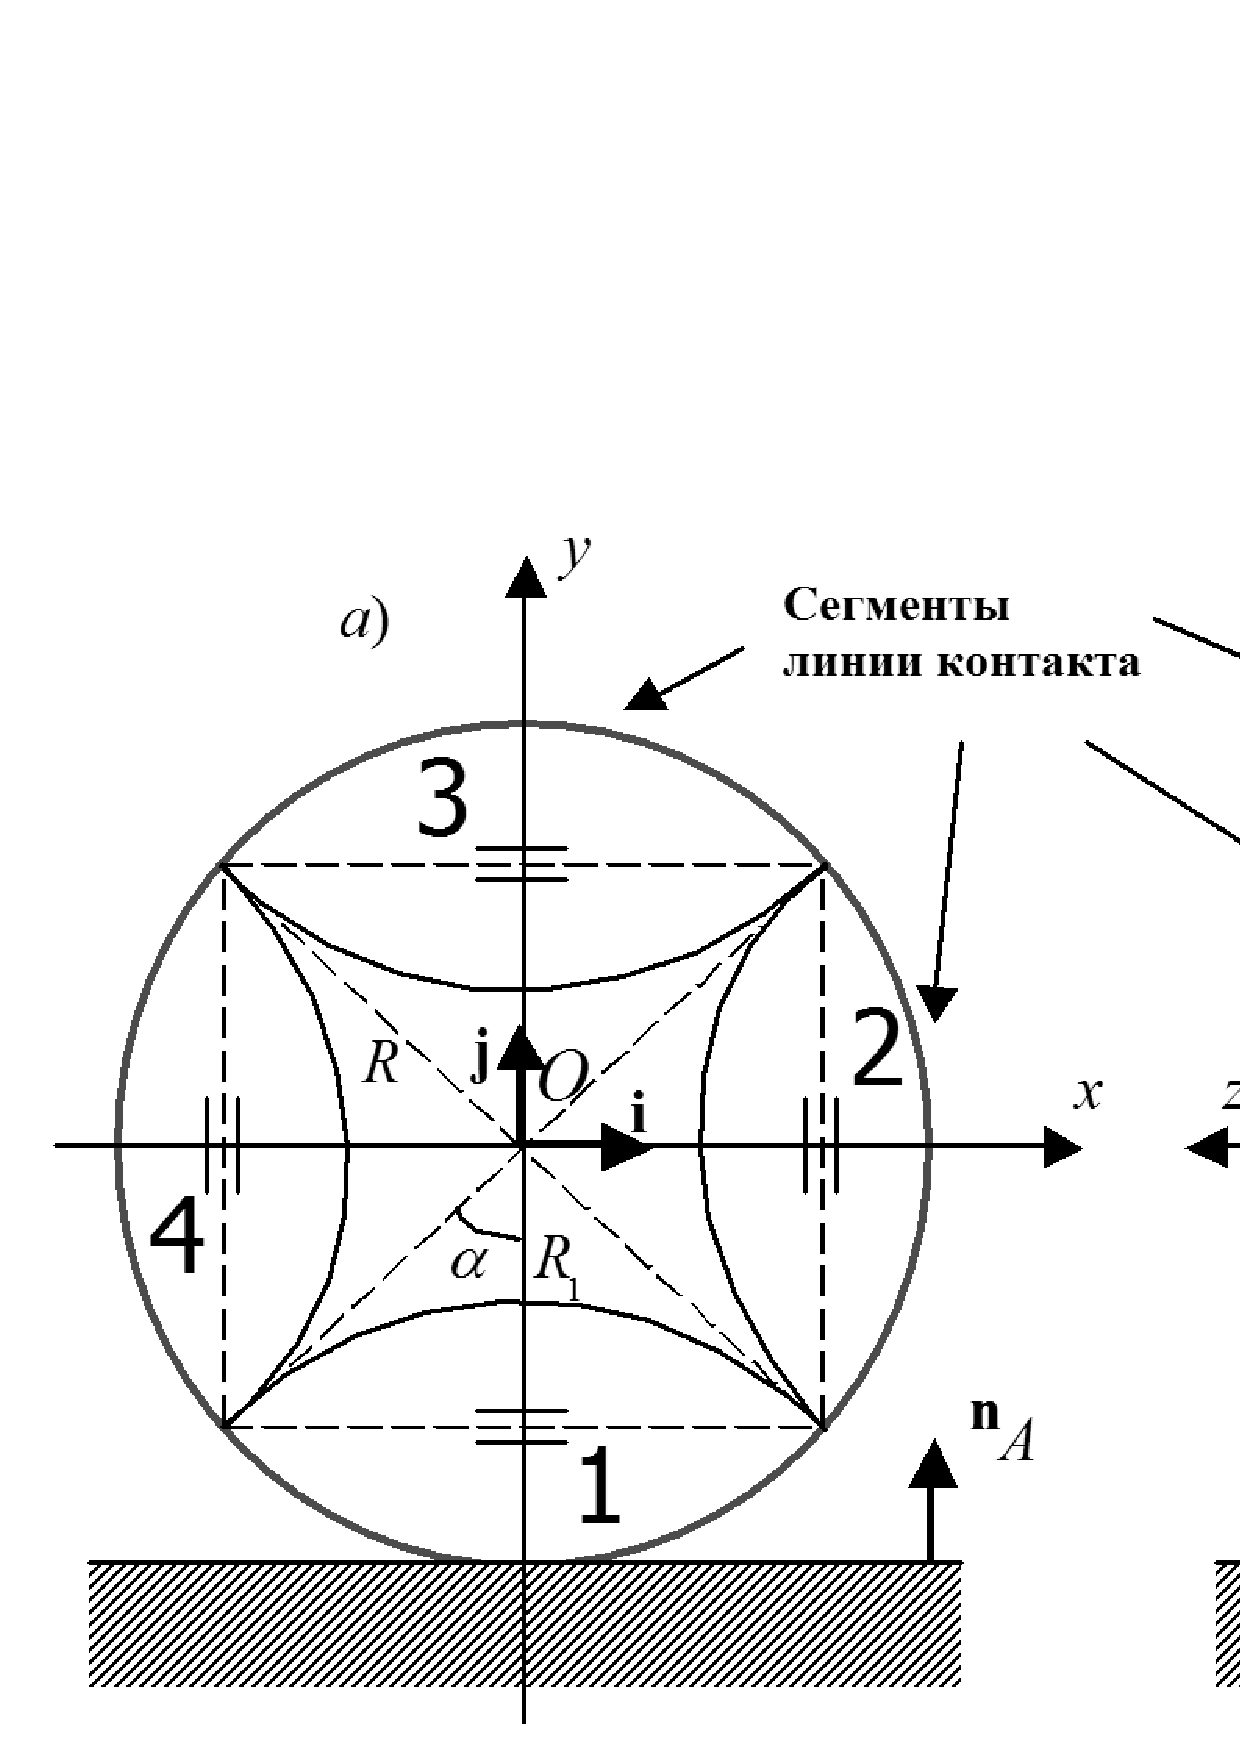
\includegraphics[bb= 0cm 0cm 20cm 15cm,scale=0.65]{OmniWheel.png}}
%\caption{Омни-колесо в вертикальном положении: a) вид сбоку; b) вид спереди.}
%\label{OmniWheel}
%\end{figure}
\begin{figure}[htb]
\centering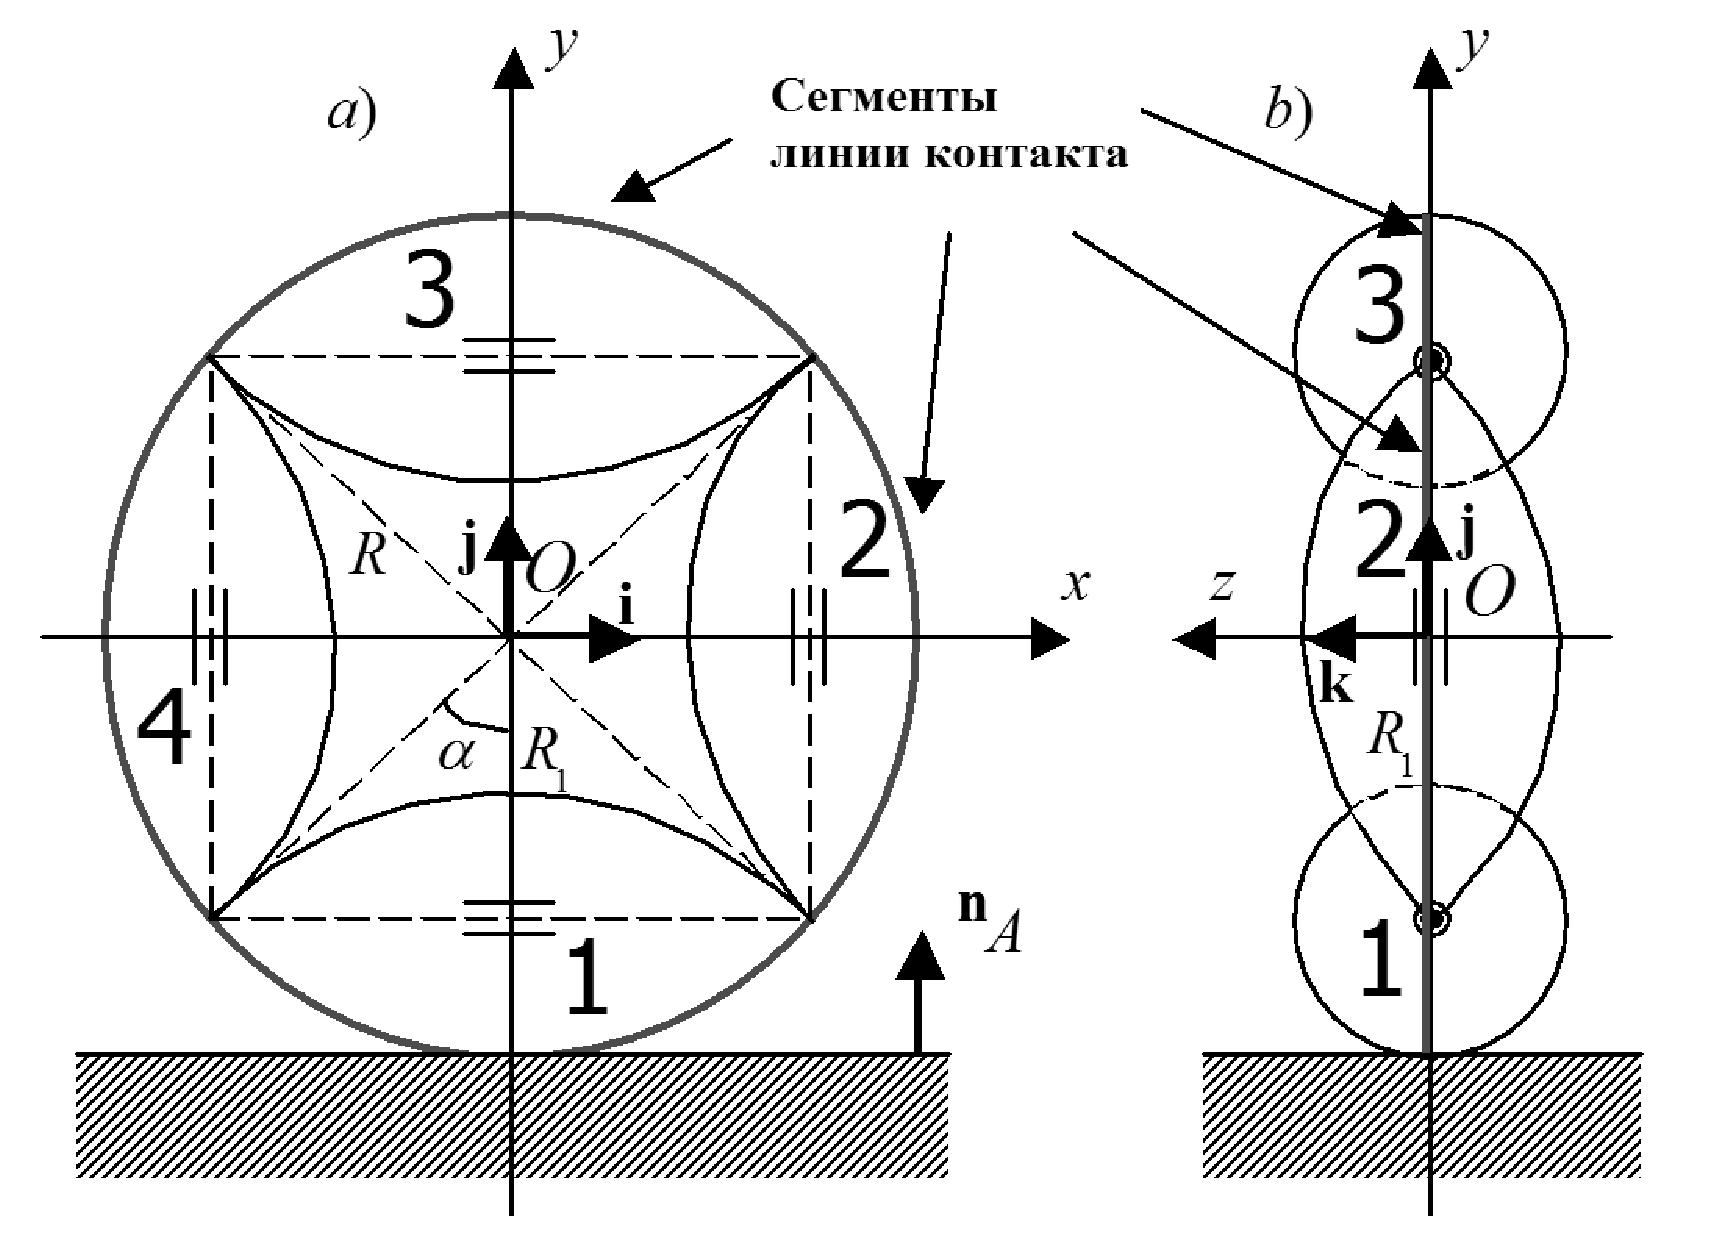
\includegraphics[width=13cm]{OmniWheel.eps}
\caption{Омни-колесо в вертикальном положении: a) вид сбоку; b) вид спереди.}
\label{OmniWheel}
\end{figure}

При описании конструкции модели омни-экипажа заметим, что количество роликов на
колесе и угол наклона оси ролика к плоскости колеса (в общем случае) являются 
параметрами модели и могут достаточно просто меняться без каких-либо 
существенных модификаций в коде самой модели. Под кодом модели мы подразумеваем
здесь её текст, написанный на языке Modelica. Фактически это список 
дифференциальных и алгебраических (включая трансцендентные) уравнений, 
возникающий неявно при работе компилятора языка, когда идет <<сборка>> 
классов-наследников в результрующий объект, представляющий динамическую модель
отдельного твердого тела или отдельную связь.

Предполагается также, что ролики размещаются на колесе таким образом, что для 
вертикально поставленного омни-колеса проекция линии контактирования наинизшего 
ролика с горизонтальной плоскостью будет состоять из последовательности 
сегментов соответствующих линий контактирования отдельных роликов. Эти сегменты 
сопрягаются таким образом, что при переходе контакта от ролика к ролику 
нормальная составляющая скорости точки ролика, находящейся в точке контакта, к 
горизонтальной плоскости равна нулю. Это означает отсутствие удара по нормали к 
плоскости. В случае коллинеарности осей роликов и плоскости колеса скачки 
скорости скольжения по касательному направлению к горизонтальной плоскости 
также отсутствуют, так как при переходе контакта между роликами их внешние 
поверхности непрерывно вырождаются в точку (в идеализированной модели), что 
означает отсутствие кинематического влияния собственного вращения роликов при 
переходе контакта с ролика на ролик. Так что в результате переключение 
контактов между роликами омни-колеса не приведет к нарушению регулярности 
движения в силу причин ударного характера. Заметим еще раз, что все описанное 
будет справедливо, если колесо все время остается в вертикальном положении.

На следующем уровне сборки модели несколько колес соединяются с подвижной 
платформой экипажа при помощи шарнирных связей. В нашем случае количество колес 
может быть три или более (в зависимости от конструкции экипажа и модели 
контактирования ролика с полом). На платформе они могут образовывать самые 
разные конфигурации. В конкретном примере Рис.~\ref{Vehicle} имеется три 
колеса, образующие равносторонний треугольник в горизонтальной плоскости $zx$. 
Ось $y$ здесь предполагается вертикальной.
%\begin{figure}[ht]
%\centerline{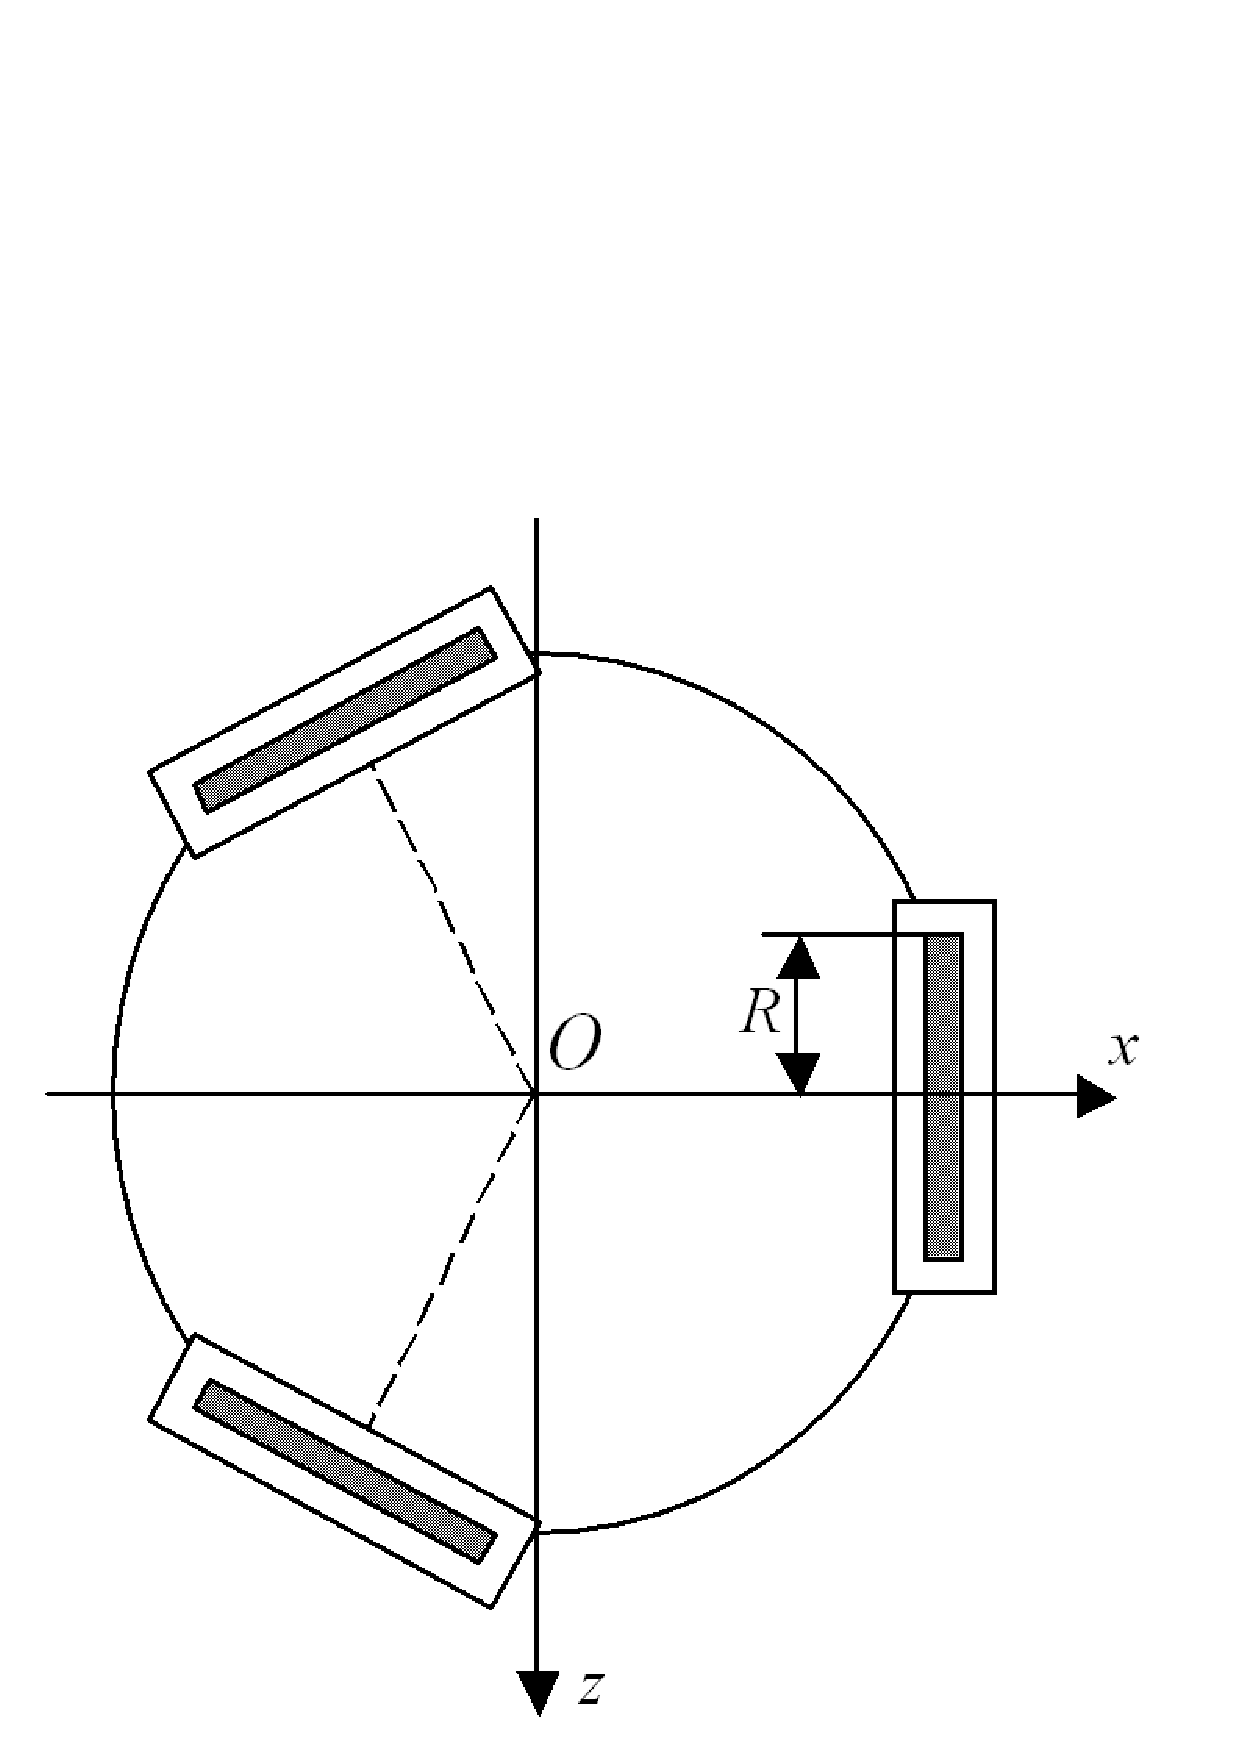
\includegraphics[bb= 0cm 0cm 20cm 21cm,scale=0.35]{Vehicle.png}}
%\caption{Трехколесный экипаж. Вид сверху.}
%\label{Vehicle}
%\end{figure}
\begin{figure}[htb]
\centering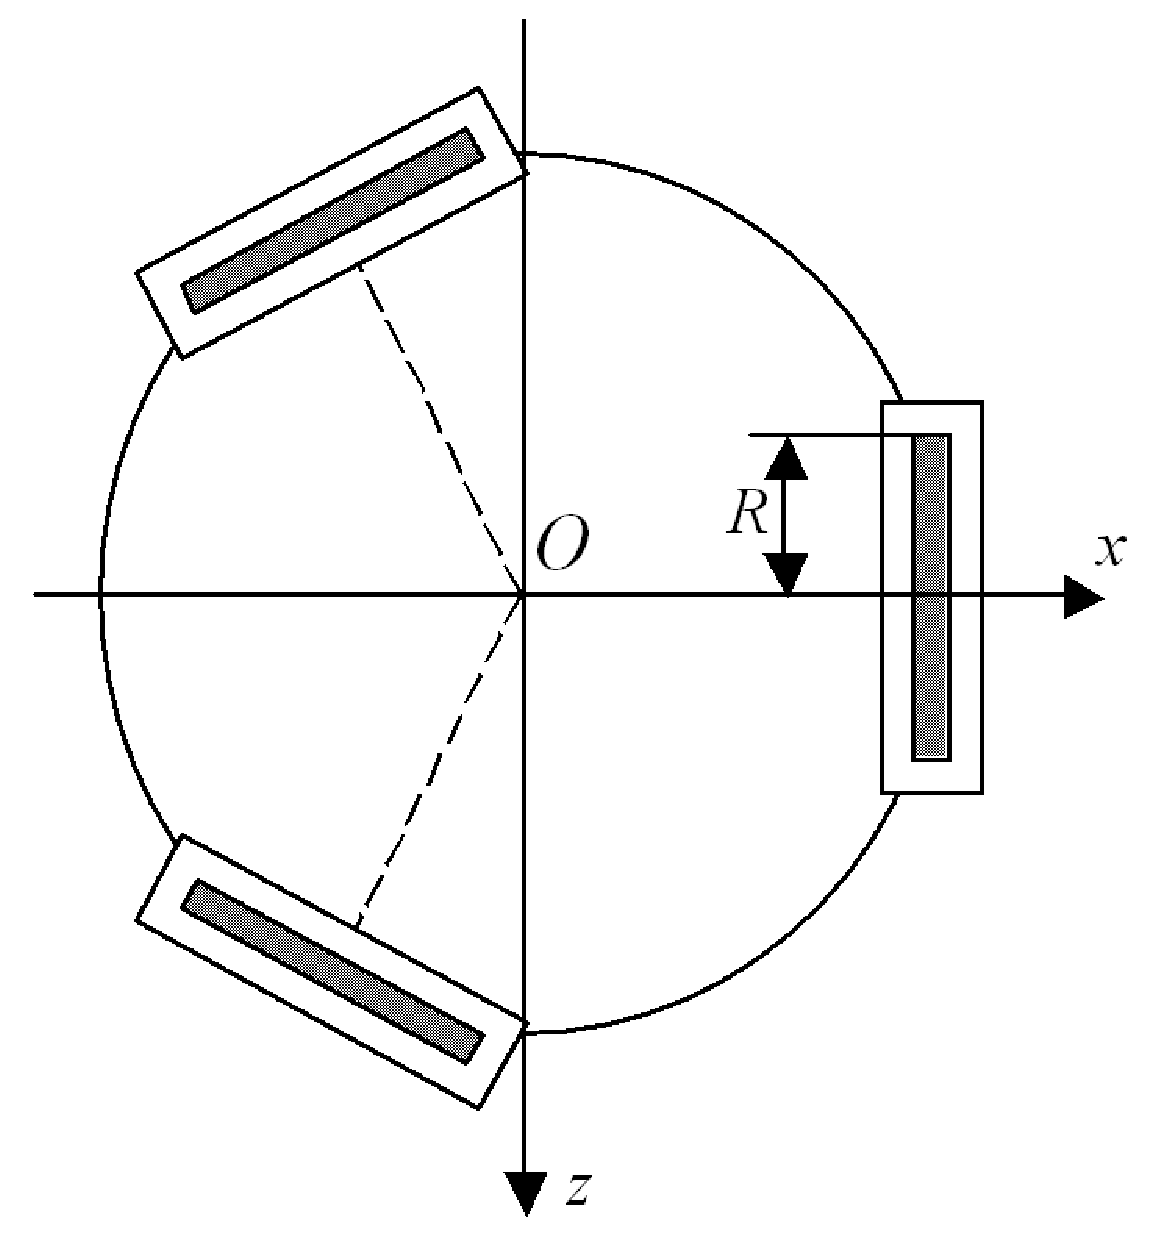
\includegraphics[width=9cm]{Vehicle.eps}
\caption{Трехколесный экипаж. Вид сверху.}
\label{Vehicle}
\end{figure}

\section{Модель динамики отдельного ролика.\ }
\label{sec3}
Вначале предположим, что ролик, представляющий собой осесимметричное 
веретенообразное твердое тело с внешней поверхностью, задаваемой в своих 
собственных осях $Oxyz$ уравнением
\begin{equation}
x^2+\left(\sqrt{y^2+z^2}+R_1\right) ^2=R^2,
\label{3_1}
\end{equation}
где $R$ --- радиус омни-колеса, $R_1=R\cos{\alpha }$ --- расстояние от центра
ролика до центра колеса, $\alpha =\pi /n$ --- половина центрального угла, под
которым ролик виден из центра колеса, $n$ --- количество роликов на колесе.
%\begin{figure}[ht]
%\centerline{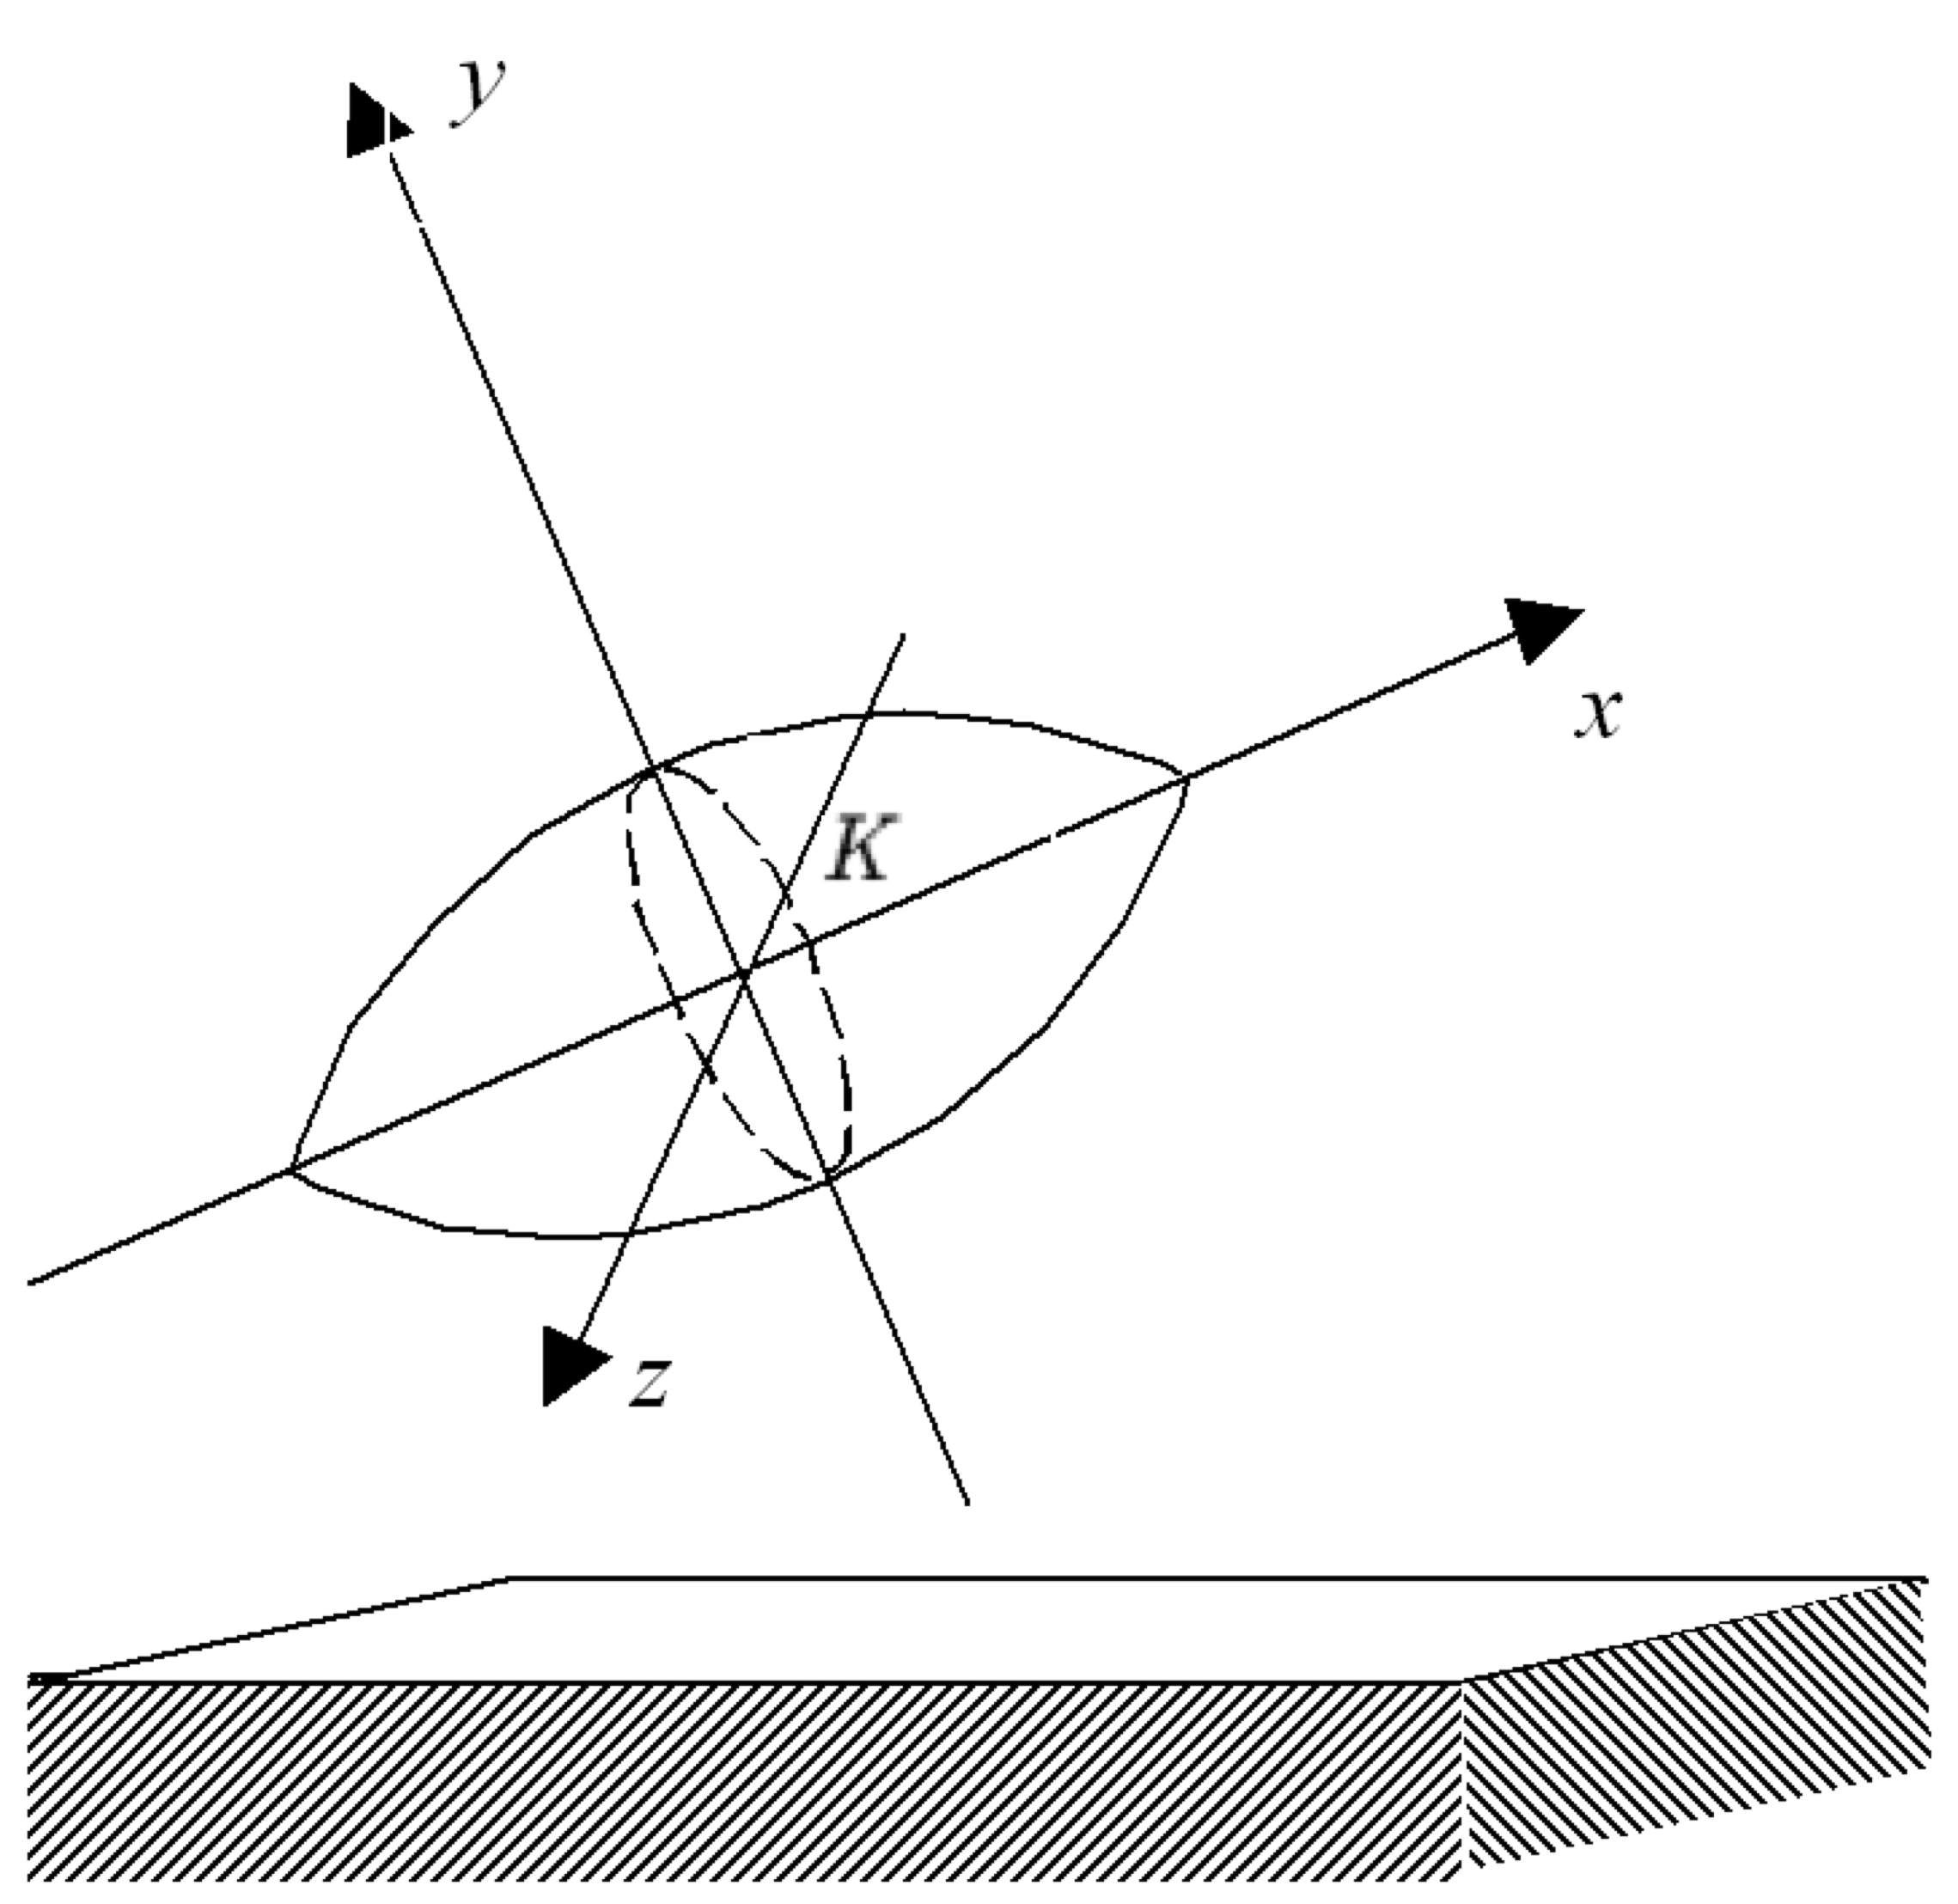
\includegraphics[bb= 0cm 0cm 20cm 21cm,scale=0.35]{Roller.png}}
%\caption{Ролик над горизонтальной плоскостью. Вид сбоку.}
%\label{Roller}
%\end{figure}
\begin{figure}[htb]
\centering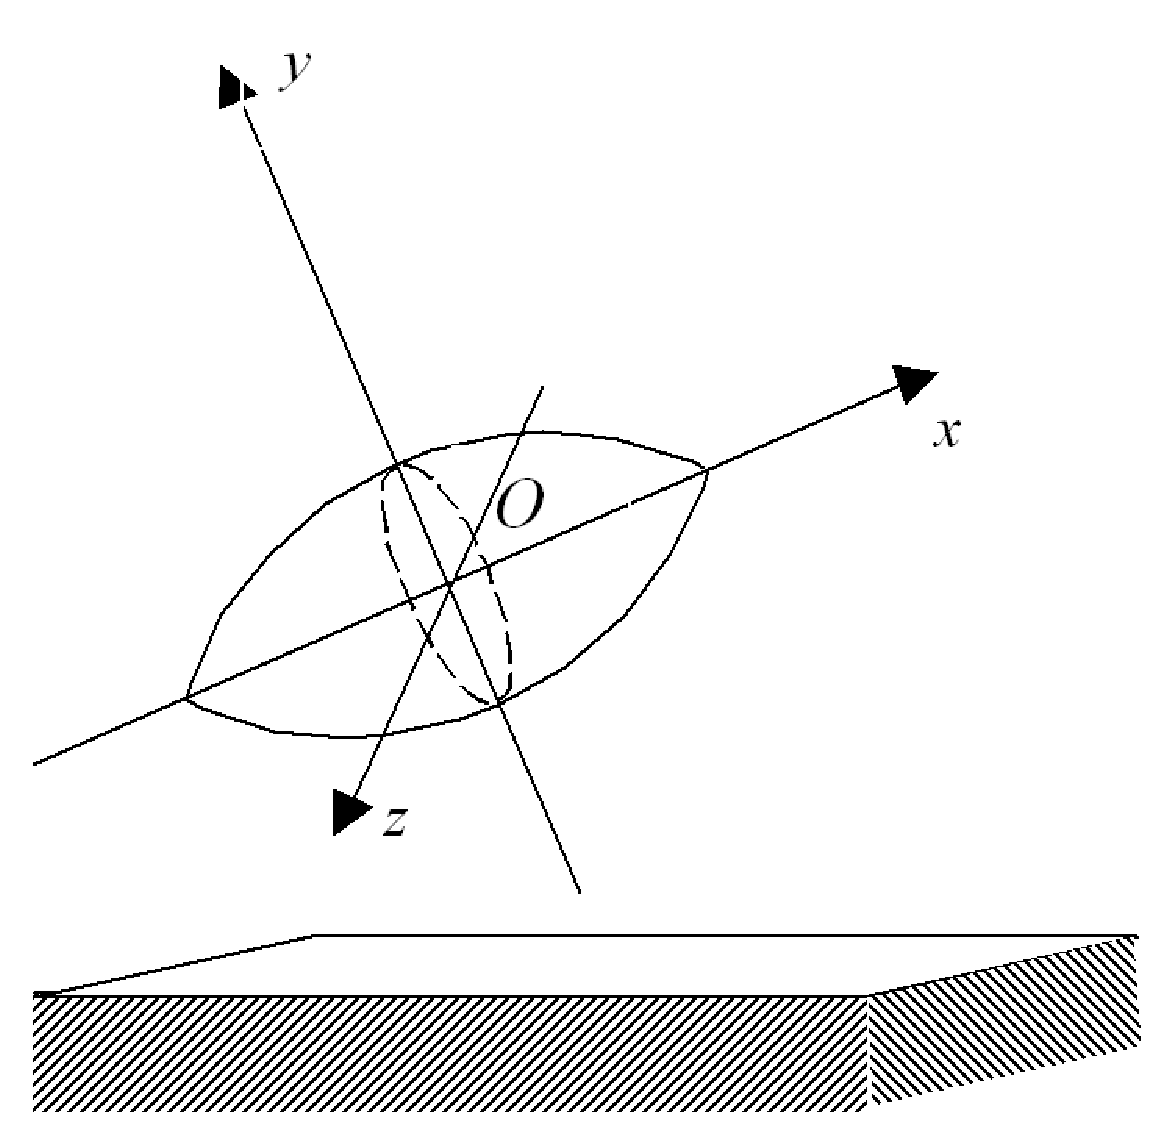
\includegraphics[width=10cm]{Roller.eps}
\caption{Ролик над горизонтальной плоскостью. Вид сбоку.}
\label{Roller}
\end{figure}

Динамика поступательно-вращательного движения реализуется так, как это описано
в~\cite{Kosenko2007}, в виде уравнений Ньютона -- Эйлера. Причем для 
моделирования вращательного движения твердого тела используется алгебра 
кватернионов~\cite{Kosenko}.

Отдельную проблему представляет задача отслеживания контакта между поверхностью 
ролика и горизонтальной плоскостью. Для моделирования динамики твердого тела с
неудерживающей связью применена технология, описанная в~\cite{Kosenko2006}. В
данном случае можно было бы применить систему алгебраических или 
дифференциально-алгебраических уравнений. Однако эти уравнения вырождаются в 
точках $x=\pm R\sin\alpha $ в координатах ролика. Такое вырождение обычно 
приводит к аварийному завершению вычислительного процесса моделирования.

В нашей задаче положение спасает специфика конфигурации, обеспечивающей 
постоянство вертикального расположения омни-колес. При этом условии можно
указать явную формулу, позволяющую вычислить ближайшую к плоскости точку $P_B$
ролика (Рис.~\ref{ContactScheme}). Этой точке всегда <<противостоит>> её 
вертикальная проекция $P_A$ на плоскость (Рис.~\ref{ContactScheme}).
%\begin{figure}[ht]
%\centerline{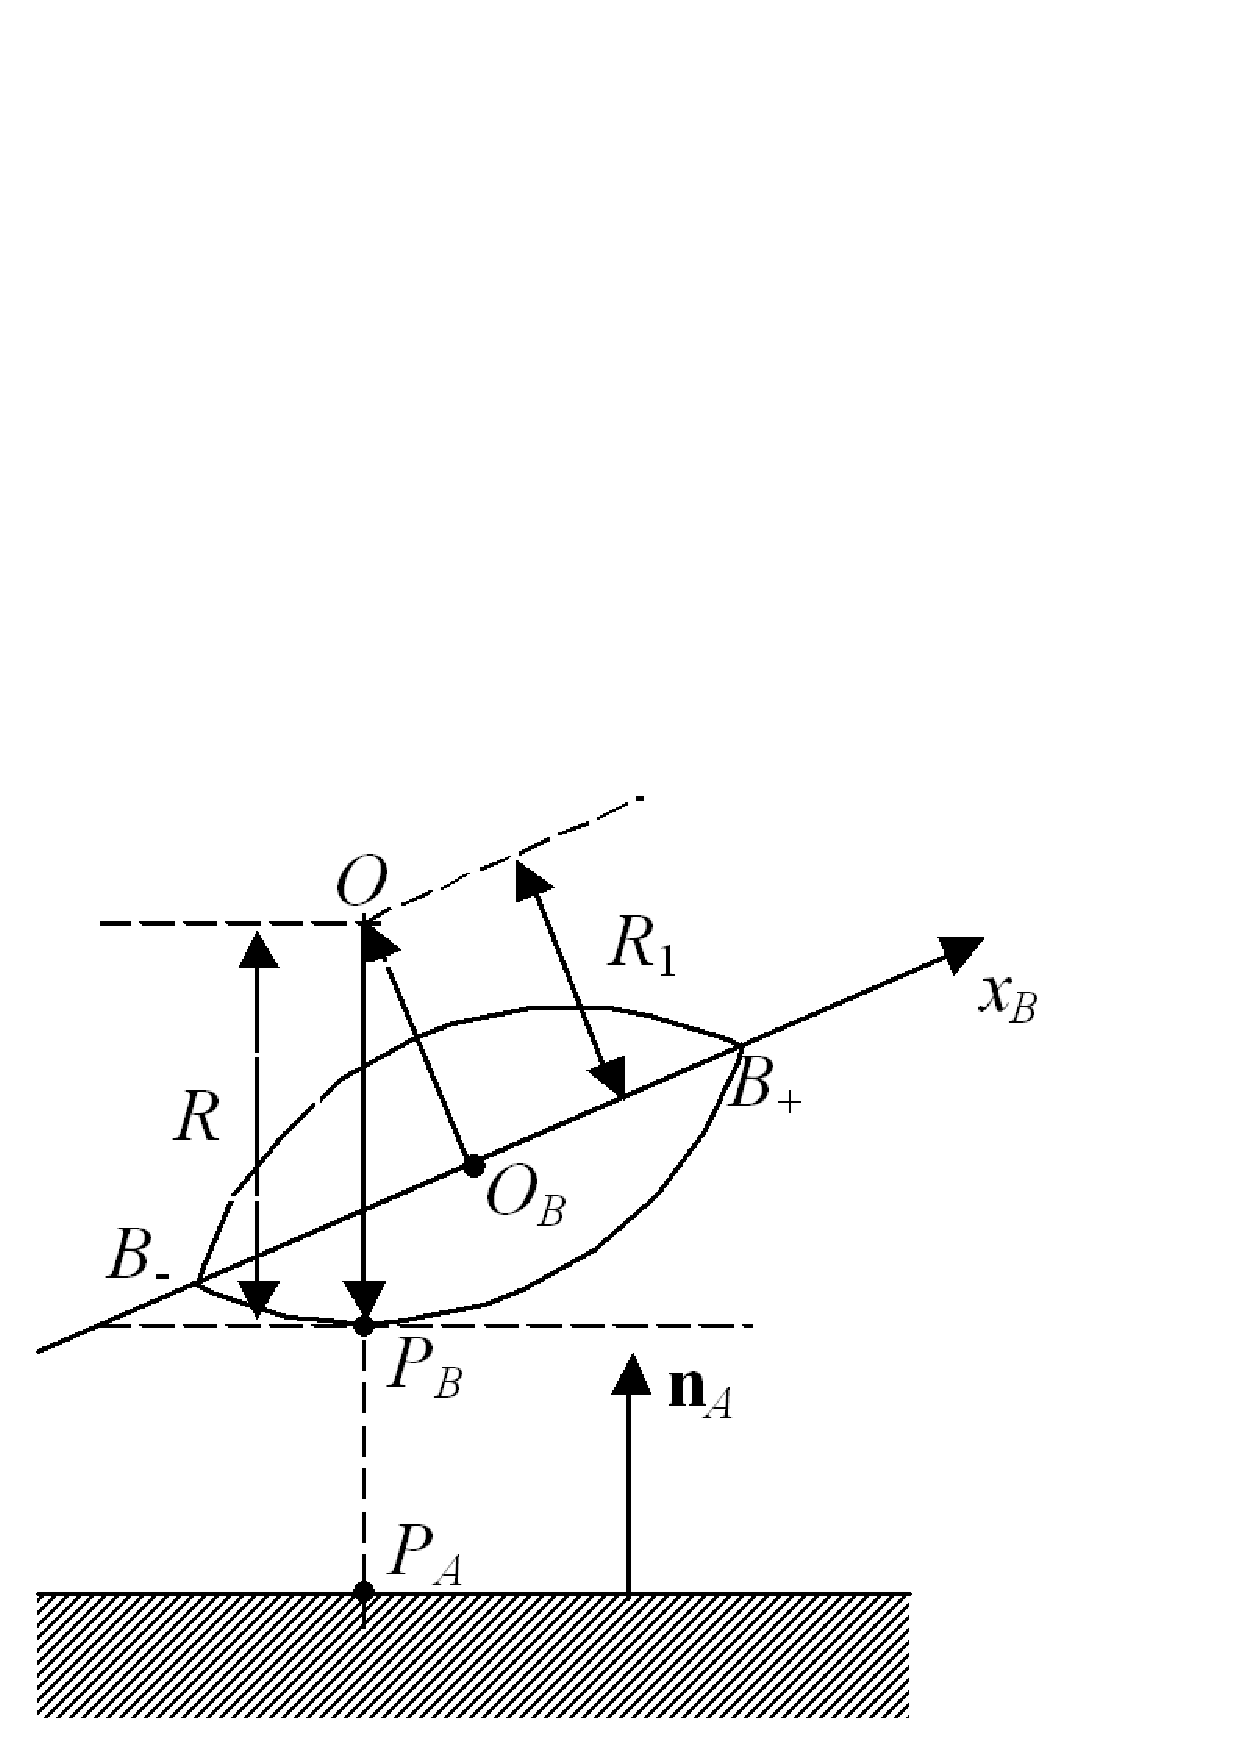
\includegraphics[bb= 0cm 0cm 20cm 21cm,scale=0.35]{RollerSection.png}}
%\caption{Схема отслеживания контакта: вид сбоку отдельного ролика.}
%\label{ContactScheme}
%\end{figure}
\begin{figure}[htb]
\centering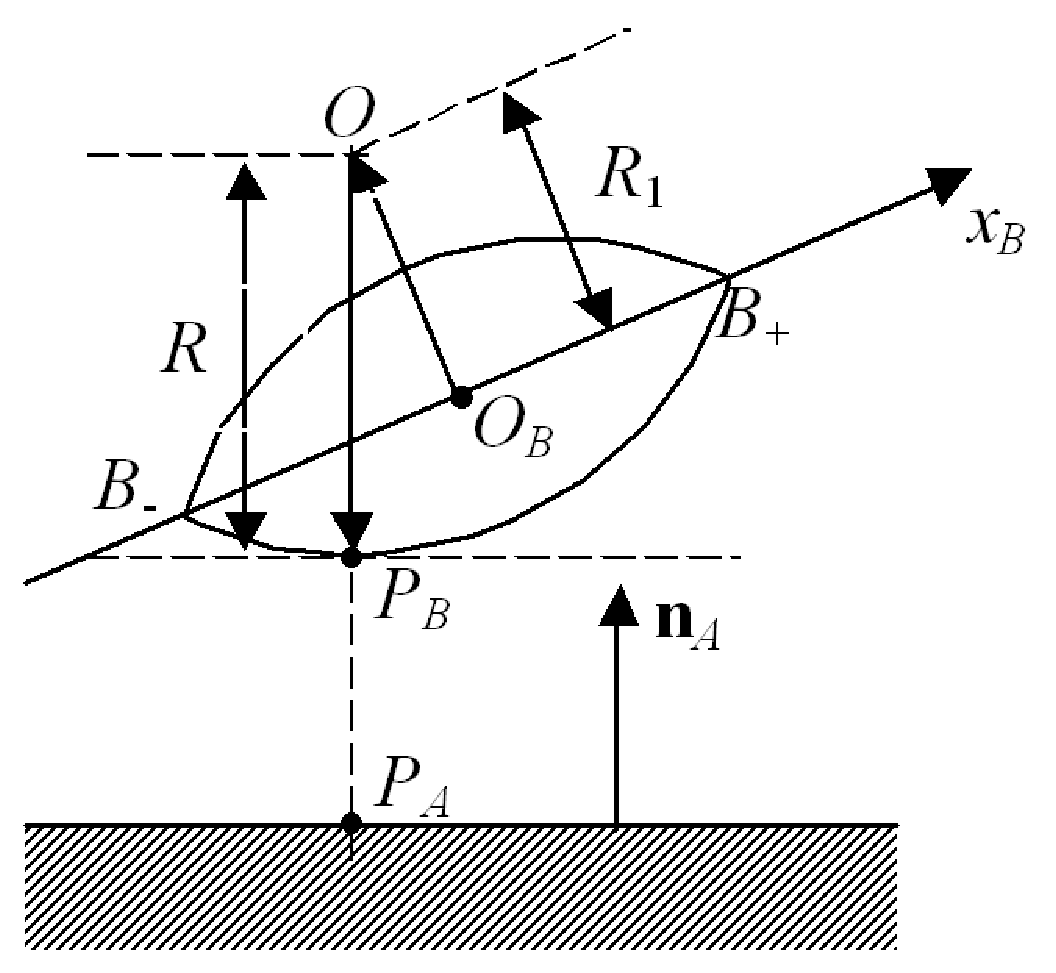
\includegraphics[width=8cm]{RollerSection.eps}
\caption{Схема отслеживания контакта: вид сбоку отдельного ролика.}
\label{ContactScheme}
\end{figure}

Обозначим символом ${\bf i}_B=(1,0,0)^T$ орт собственной оси ролика $O_Bx_B$.
Этот вектор представлен в системе координат ролика $O_Bx_By_Bz_B$. Пусть $T_B$
--- матрица поворота ролика относительно инерциальной системы координат 
$O_Ax_Ay_Az_A$, связанной с неподвижной плоскостью. Пусть также ${\bf r}_B$ ---
радиус-вектор геометрического центра ролика в текущий момент времени и 
${\bf n}_A=(0,1,0)^T$ --- орт нормали (восходящей вертикали) к плоскости. 
Плоскость условно обозначается нами телом с индексом $A$, ролик --- $B$. Пусть
${\bf d}$ --- горизонтальный орт, вычисляемый по формуле
$$
{\bf d}=\dfrac{T_B{\bf i}_B\times {\bf n}_A}
              {\left| T_B{\bf i}_B\times {\bf n}_A\right|}.
$$
Тогда, очевидно, отрезок $\overrightarrow{O_BO}$, расположенный в вертикальной
плоскости, будет иметь длину $R_1$ и задаваться формулой
$$
\overrightarrow{O_BO}=R_1{\bf d}\times T_B{\bf i}_B.
$$
Здесь $O$ --- центр кривизны окружности вертикального сечения ролика 
(Рис.~\ref{ContactScheme}). Так что самая нижняя точка $P_B$ внешней 
поверхности ролика будет задаваться по формуле
\begin{equation}
{\bf r}_{P_B}={\bf r}_B+R_1{\bf d}\times T_B{\bf i}_B-R{\bf n}_A,
\label{3_2_0}
\end{equation}
поскольку точка $P_B$ лежит на упоминавшейся выше окружности на общей вертикали 
с точкой $O$. Для вычисления положения точки $P_A$ нужно вторую координату 
вектора ${\bf r}_{P_B}$ положить равной нулю
\begin{equation}
{\bf r}_{P_A}=\left( x_{P_B},0,z_{P_B}\right) ^T.
\label{3_2_1}
\end{equation}

Вся описанная выше вычислительная процедура будет справедлива только, если 
вектор $T_B{\bf i}_B$ имеет направление, ограниченное по вертикали углами
$\pm\alpha $. Если соответствующий угол превышает значение $\alpha $, то 
следует положить $P_B=B_{-}$, где $B_{-}$ --- левая концевая точка ролика. Если
же этот угол меньше величины $-\alpha $, нужно положить $P_B=B_{+}$, где 
$B_{+}$ --- правая концевая точка ролика.

В конечном итоге условие контактирования ролика и плоскости можно записать в 
виде
\begin{equation}
\left| T_B{\bf i}_B\cdot {\bf n}_A\right|\le\sin\alpha .
\label{3_2}
\end{equation}
Это условие, однако, позволяет из всего множества роликов колеса выделить 
нижний (контактирующий) и верхний. Чтобы отбросить случай последнего ролика
можно к последнему условию присоединить также требование 
\begin{equation}
y_B<R,
\label{3_3}
\end{equation}
где $y_B$ --- высота центра ролика относительно инерциальной системы координат.

Таким образом, конъюнкция условий (\ref{3_2}) и (\ref{3_3}) означает наличие
контакта. В противном случае, при отсутствии контакта, нормальная реакция 
отсутствует (закон Синьорини). С другой стороны, реализация контакта 
геометрически означает выполнение скалярного условия 
\begin{equation}
y_{P_B}=0,
\label{3_4}
\end{equation}
а его отсутствие --- также скалярного (альтернативного) условия
$$
F_n=0,
$$
где $F_n$ --- нормальная составляющая реакции (в данном случае отсутствующей) 
приложенной в точке $P_B$.

Вычислительная практика показала, что уравнения контакта в форме (\ref{3_4})
стабильно приводит к аварийному завершению процесса симуляции динамической 
модели ролика. Аналогичный результат получается, если в качестве уравнения 
контактирования использовать уравнение вида 
$$
v_n=0,
$$
где $v_n$ --- нормальная составляющая скорости точки контактирования, лежащей
на теле $B$, относительно тела $A$ (горизонтальной плоскости). И только 
уравнение вида
$$
\dot{v}_n=0
$$
приводит к требуемому результату --- корректной работе объекта контактирования
(реализованного в данном случае на языке Modelica~\cite{Fritzson}) в процессе 
симуляции модели. Заметим, что вся реализация процесса контактирования 
выполнена в предположении точечного <<твердого>> контакта твердых тел без 
какой-либо податливости.

Для каждого ролика модели омни--экипажа при контактировании <<включается>>
используемая здесь модель трения. Это <<простейший>> закон Амонтона -- Кулона
сухого трения. На самом деле вместо этого нами используется кусочно--линейная 
аппроксимация точного закона трения~\cite{Kosenko2006}. Эта аппроксимация 
обеспечивает высокую точность вычисления движения тел на больших интервалах 
времени~\cite{Novozhilov}. Заметим, что и в общем случае реализация модели 
неудерживающей связи основывается на результатах, обозначенных в 
работе~\cite{Kosenko2006}.

\section{Модель сборки первого уровня: омни--колесо.\ }
\label{sec4}
Процесс сборки виртуального прототипа омни--экипажа реализуется за два шага:
а) сборка виртуального прототипа омни--колеса, состоящего из собственно колеса
и набора роликов, присоединенных к нему; б) сборка виртуального прототипа
экипажа при помощи операции инстанциации (установки объекта класса) объектов 
класса омни--колеса этапа а) в контейнерный класс прототипа экипажа.

%\begin{figure}[ht]
%\centerline{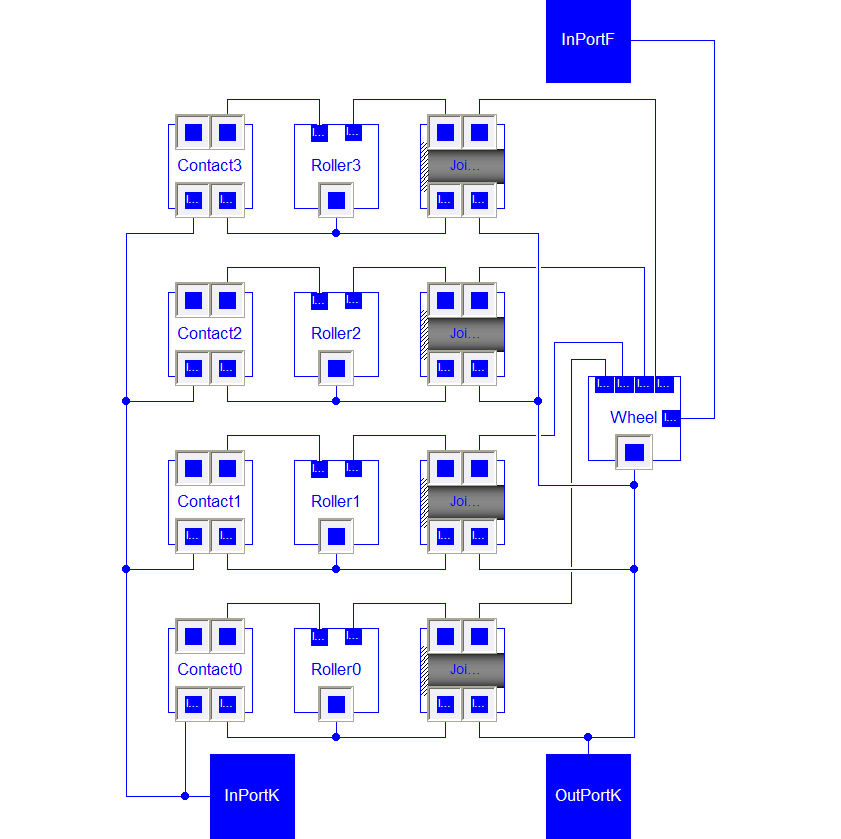
\includegraphics[bb= 0cm 0cm 20cm 20cm,scale=0.7]{OmniWheelModel.png}}
%\caption{Визуальная модель омни--колеса.}
%\label{OmniWheelModel}
%\end{figure}
\begin{figure}[htb]
\centering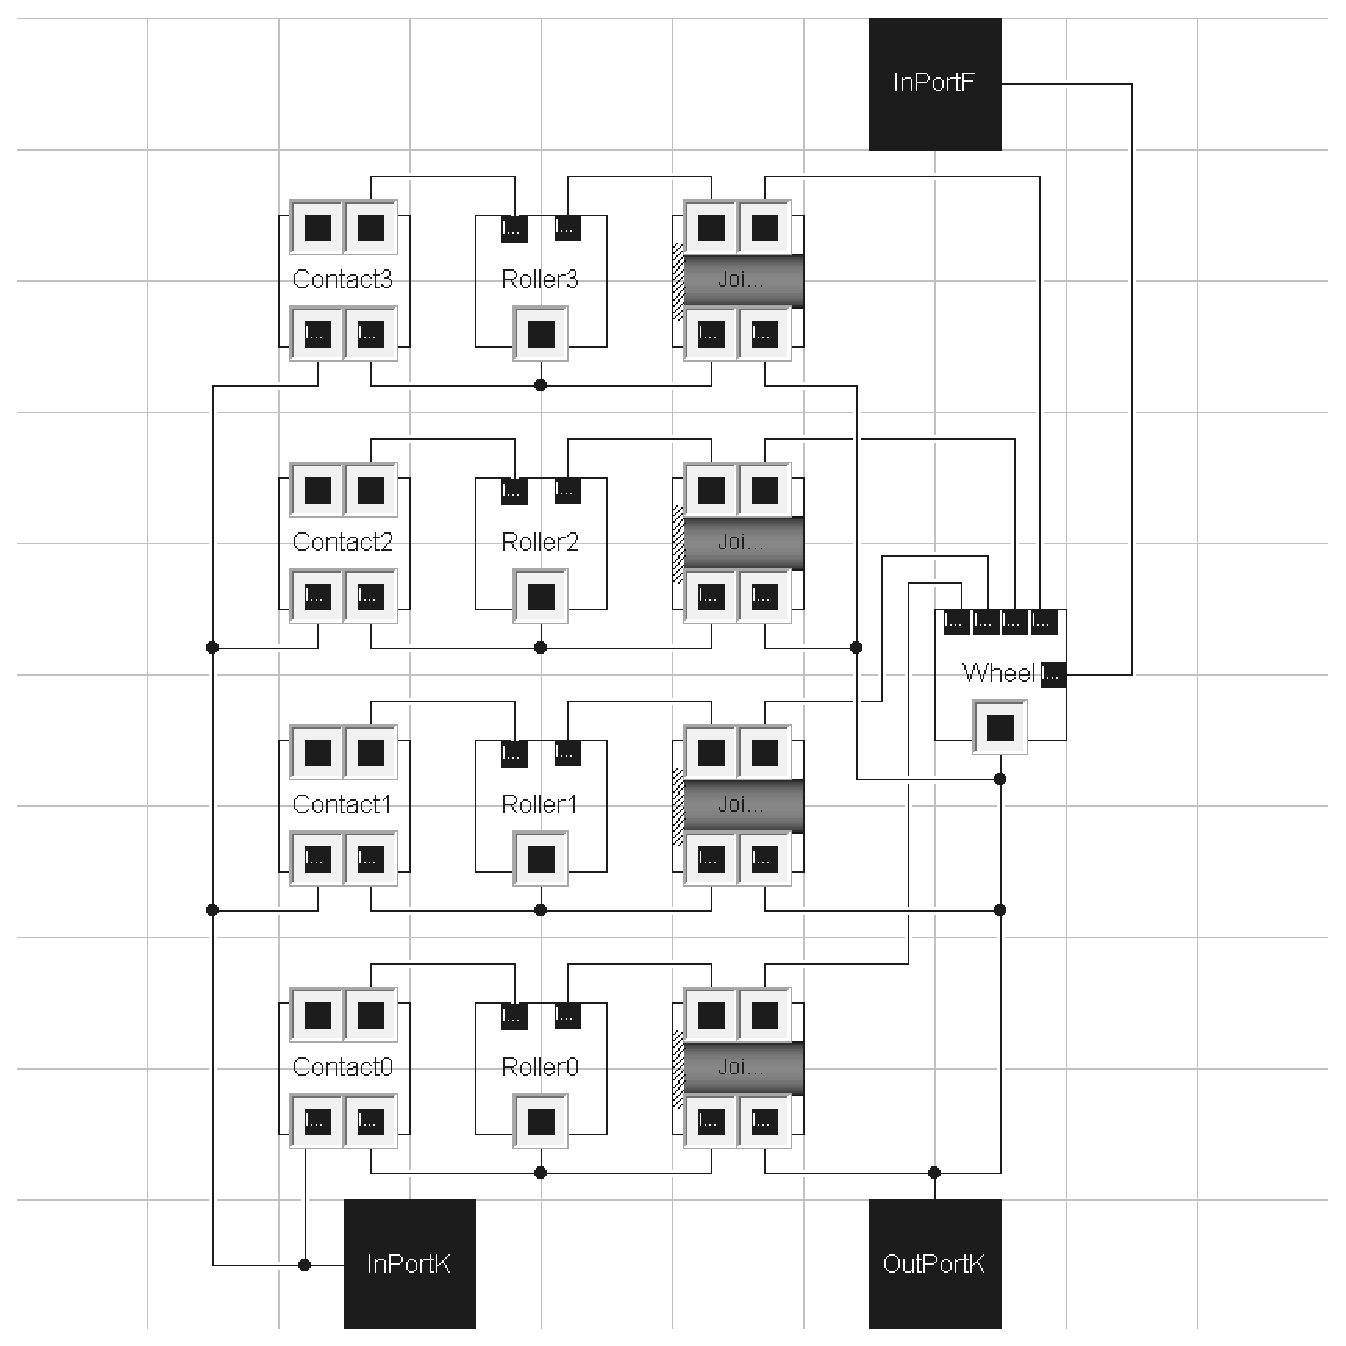
\includegraphics[width=15cm]{OmniWheelModel.eps}
\caption{Визуальная модель омни--колеса.}
\label{OmniWheelModel}
\end{figure}

Для сборки $n$ роликов колеса (в нашем примере мы для определенности полагаем
$n=4$) мы использовали ранее развитую технику реализации шарнирных связей
различных типов~\cite{Kosenko2007}. В данном случае используется класс, 
задающий шарнир, обеспечивающий свободное относительное вращение одного тела
(ролика) относительно другого тела (колеса). Одновременно не допускается 
(поступательное) относительное перемещение тел вдоль оси шарнира. Визуальная 
модель омни--колеса изображена на Рис.~\ref{OmniWheelModel}. Дадим здесь более
подробное описание этой модели.

Вначале рассмотрим абстрактную схему информационных коммуникаций для одной,
отдельно взятой, механической связи. Эта схема показана на 
Рис.~\ref{ConstraintScheme}. Здесь $A$ и $B$ --- идентификаторы моделей двух 
твердых тел, взаимодействующих при помощи объекта связи. Общая схема такова: 
модели динамики тел $A$ и $B$, содержащие дифференциальные уравнения 
поступательно-вращательного движения в каждом экземпляре ($A$ и $B$) класса
<<Твердое тело>> при помощи численных интеграторов вырабатывает кинематическую
информацию о положении тел, их ориентации, скоростях и ускорениях. Вся эта 
информация у каждого из тел непрерывно поступает на экспорт из объектов $A$ и 
$B$ через соответствующий кинематический порт. У объекта тела имеется в 
точности один кинематический порт.

%\begin{figure}[ht]
%\centerline{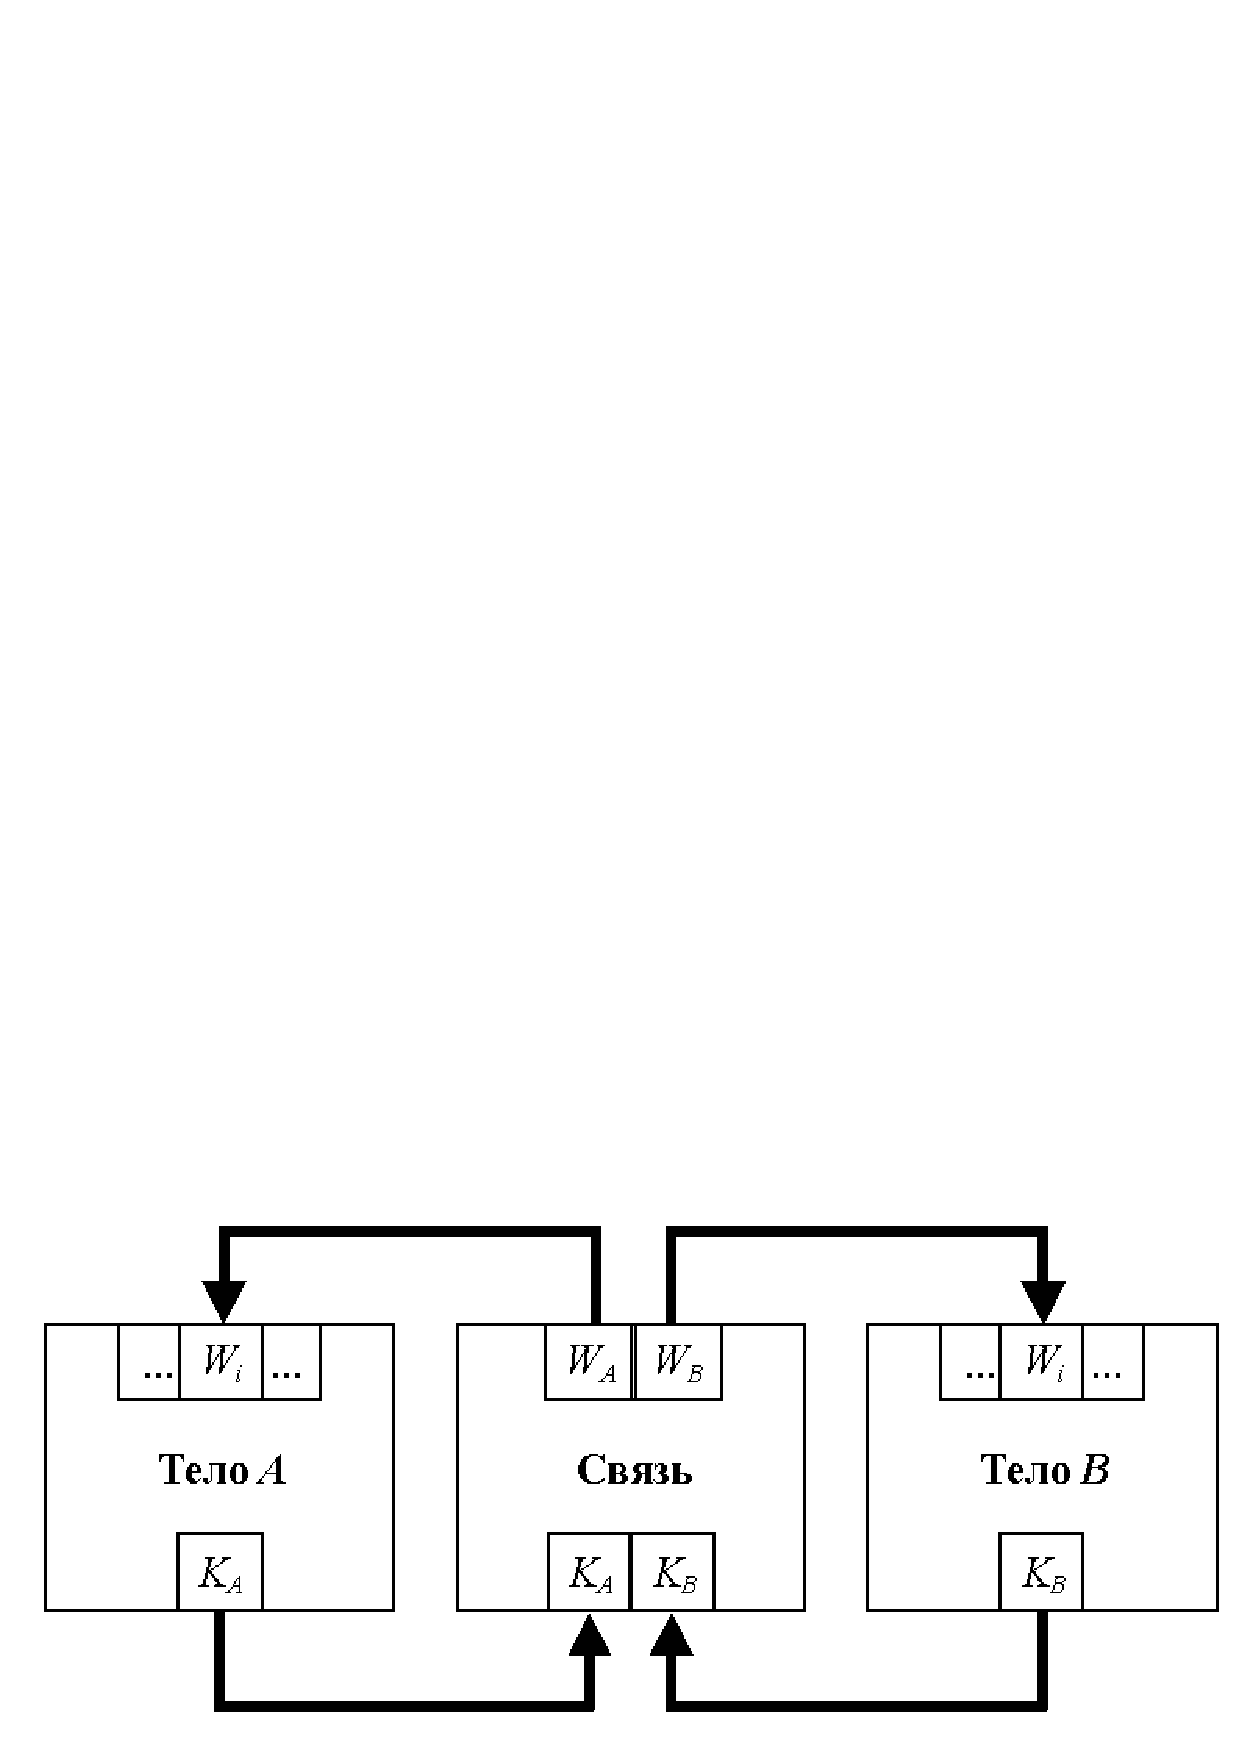
\includegraphics[bb= 0cm 0cm 20cm 8cm,scale=0.7]{Fig_2_1.png}}
%\caption{Коммуникационная сеть механической связи.}
%\label{ConstraintScheme}
%\end{figure}
\begin{figure}[htb]
\centering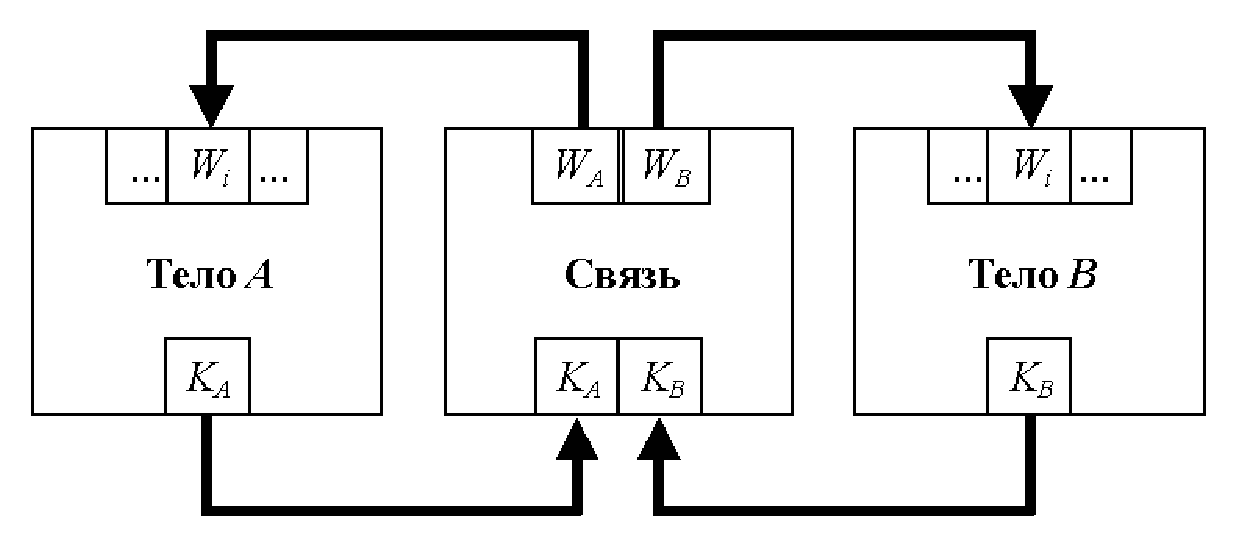
\includegraphics[width=14cm]{Fig_2_1.eps}
\caption{Коммуникационная сеть механической связи.}
\label{ConstraintScheme}
\end{figure}

Кинематическую информацию от тел $A$ и $B$ также непрерывно во времени 
импортирует объект связи через два входных порта (Рис.~\ref{ConstraintScheme})
Внутри объекта связи эта информация (соответствующие переменные) 
<<пропускается>> через систему уравнений данного конкретного вида механической
связи. При этом объект связи <<вырабатывает>> и экспортирует через свои 
выходные силовые порты пары вида (<<сила>>, <<момент>>) = <<силовой мотор>>. 
Эта информация через два выходных порта поступает на вход в объекты $A$ и $B$.

Таким образом, коммуникационная сеть механической связи <<замыкается>>. Набор 
указанных пар взаимодействующих тел и составляет модель динамики систем тел. В
визуальных моделях омни-колеса и экипажа легко угадываются такие 
<<элементарные>> ячейки взаимодействия тел, на которые наложены механические 
ограничения (связи). Рассмотрим для определенности механическую систему 
омни-колеса (Рис.~\ref{OmniWheelModel}). Но сначала обратим внимание на 
визуальную модель экипажа (Рис.~\ref{OmniVehicle}). Здесь слева расположен 
объект базового тела --- горизонтального пола. Этот объект не имеет динамики.
Имеется только заданная кинематическая информация.

%\begin{figure}[ht]
%\centerline{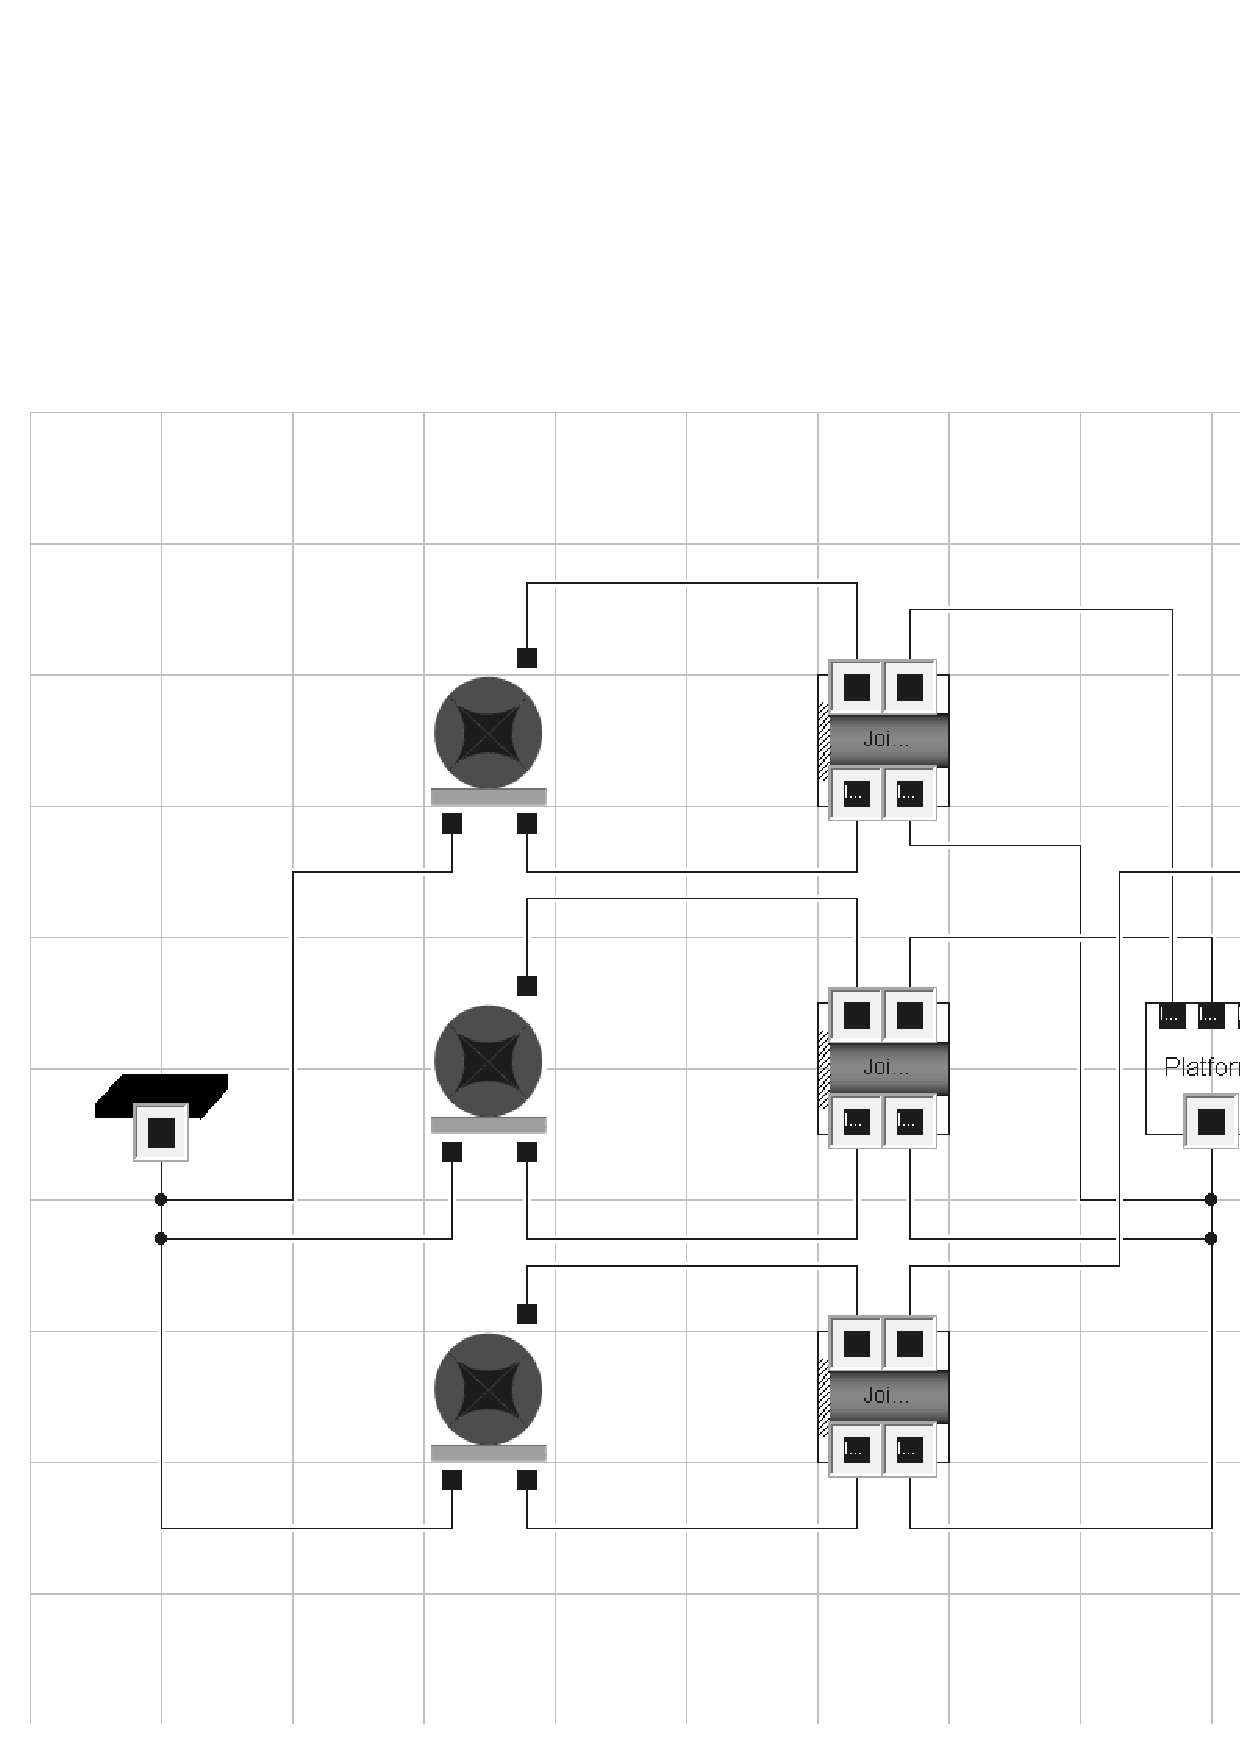
\includegraphics[bb= 0cm 0cm 20cm 20cm,scale=0.7]{OmniVehicleModel.png}}
%\caption{Визуальная модель омни--экипажа.}
%\label{OmniVehicle}
%\end{figure}
\begin{figure}[htb]
\centering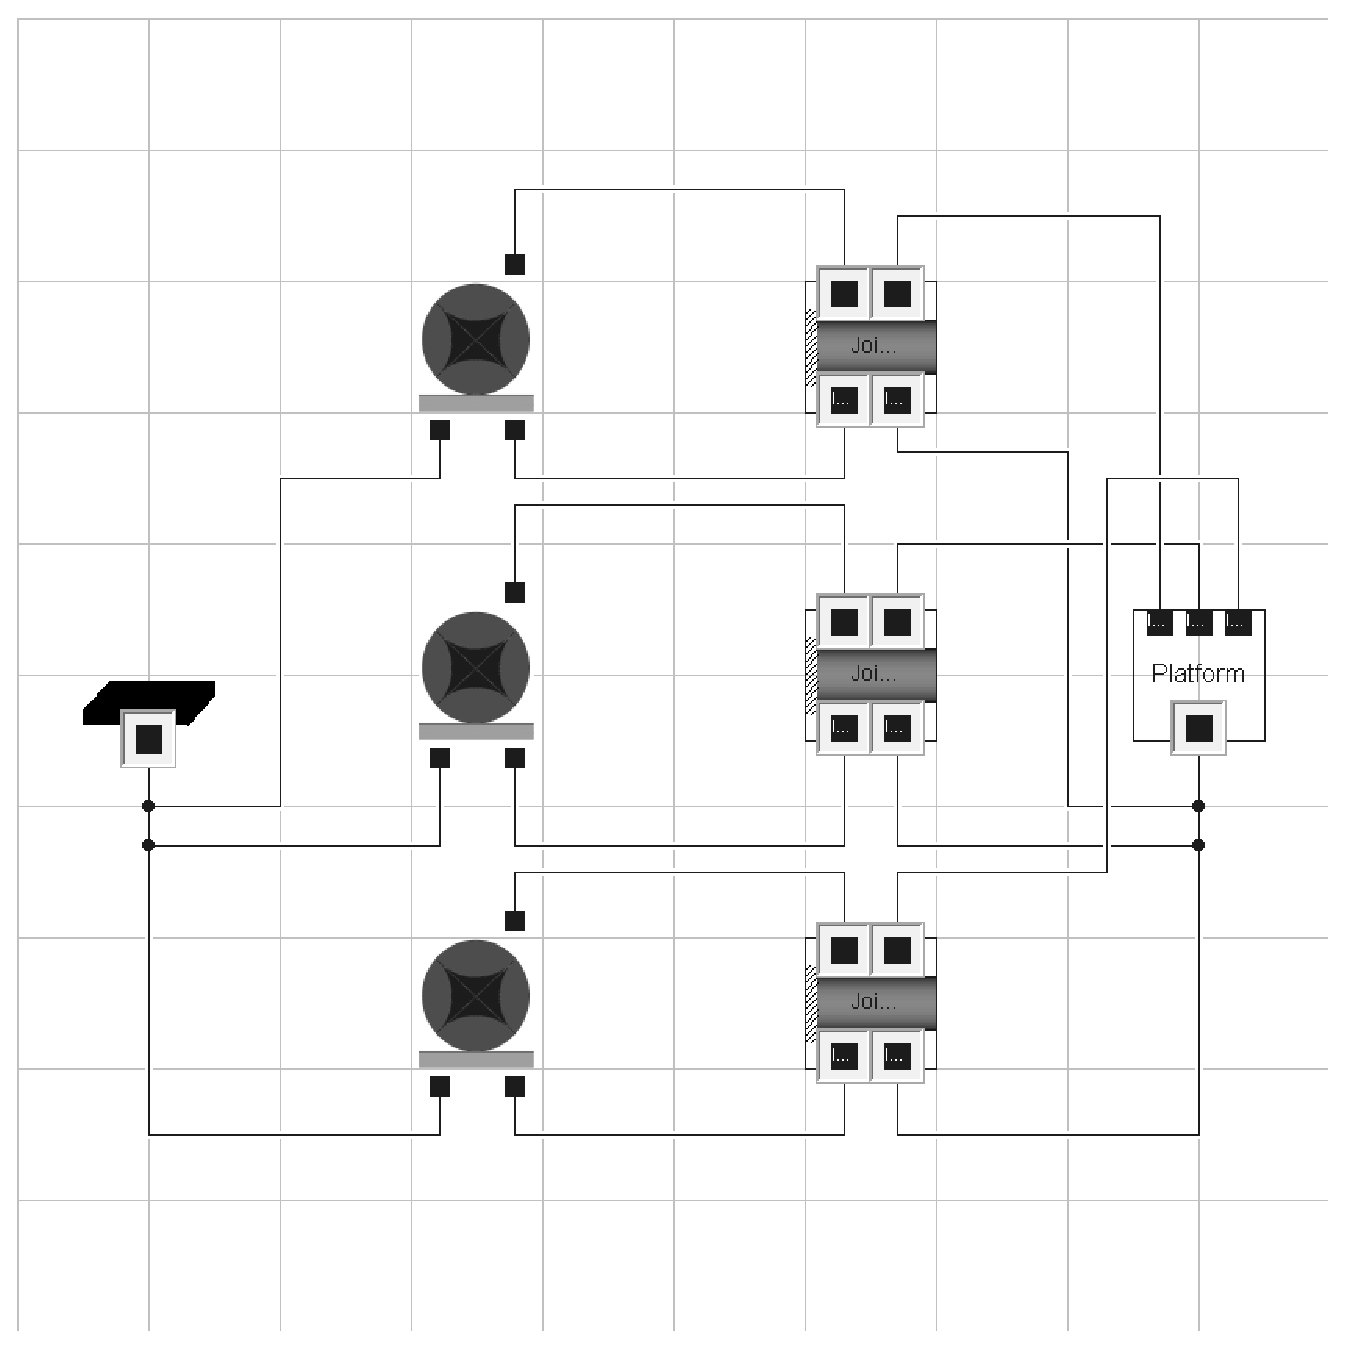
\includegraphics[width=15cm]{OmniVehicleModel.eps}
\caption{Визуальная модель омни--экипажа.}
\label{OmniVehicle}
\end{figure}

Базовое тело и каждый из роликов омни-колеса находятся в контактном 
взаимодействии. Это взаимодействие реализуется при помощи порта $InPortK$
(Рис.~\ref{OmniWheelModel}), три экземпляра которого мы можем видеть на схеме
Рис.~\ref{OmniVehicle}. Здесь реализована неудерживающая связь, обеспечивающая 
в нашем конкретном случае точечный твердотельный контакт поверхности ролика и
поверхности пола. Причем, конструкция омни-колеса такова, что в каждый данный 
момент времени имеется имеется только один контакт. Остальные ролики <<висят>>
над полом. При этом механическая связь между полом и, <<висящим>> на ободе
колеса, роликом не исчезает --- алгоритм отслеживания контакта продолжает 
работать, генерируя в качестве реакций нулевые усилия и моменты.

В случае фактического выполнения контакта помимо нормальной реакции вычисляется
также её касательная составляющая, симулирующая силу трения. Для касательного 
контактного усилия имеется (как и для нормального) множество различных моделей. 
Мы остановились на реализации простейшего случая --- модели сухого трения при 
одноточечном твердотельном контакте. При этом, как известно~\cite{Novozhilov}, 
идеальный <<сухой>> случай реализовать не удается. Вместо разрывной функции 
sign от касательной скорости относительного скольжения контактирующих 
поверхностей используется её регуляризованный в нуле вариант. В нашем случае 
вместо функции знака sign применяется функция линейного насыщения, имеющая в 
окрестности нуля <<крутой>> линейный участок. Для таких функций известен 
результат~\cite{Novozhilov} о близости аппроксимирующего движения и движения, 
соответствующего <<точному>> случаю разрывной функции sign.

Обращаясь далее к визуальной модели омни-колеса, видим, что каждый из роликов 
соединен с ободом колеса при помощи цилиндрического шарнира (объекты связей
$Joint0,\dots ,Joint3$). Это модели шарниров, которые обеспечивают свободное
вращение роликов относительно корпуса колеса.

Кроме описанных объектов, составляющих модель динамики омни-колеса, эта модель
имеет порты своих внешних связей. Это уже упомянутый выше порт $InPortK$ связи
с базовым телом, а также порты $OutPortK$ (кинематика), $InPortF$ (усилия) 
соединений с шарнирами монтажа колес и корпуса всего экипажа (показаны на 
визуальной модели экипажа на Рис.~\ref{OmniVehicle}). Заметим здесь же, что 
каждый из объектов визуальной модели имеет набор соответствующих уравнений
(дифференциальных и/или алгебраических), порожденных из класса данного объекта.

В процессе отладки модели рассматривались автономные движения отдельного 
омни-колеса. Наибольший интерес представляет сборочный уровень всего экипажа
(Рис.~\ref{Vehicle}). Соединительные устройства были также реализованы как 
объекты того же самого шарнирного класса из шага а). Эти шарниры соединяют 
корпус экипажа и каждое из колес. Все упомянутые шарниры <<разрешают>> 
относительное вращение без какого-либо сопротивления и одновременно блокируют
скольжение вдоль оси шарнира. Визуальная модель экипажа показана на 
Рис~\ref{OmniVehicle}. Здесь для наглядности объекты показаны в виде скалярных
элементов. На самом деле при произвольном $n$ и произвольном числе и 
расположении колес следует использовать массивы объектов класса <<ролик>> и 
класса <<омни--колесо>>.

\begin{figure}[htb]
\centerline{
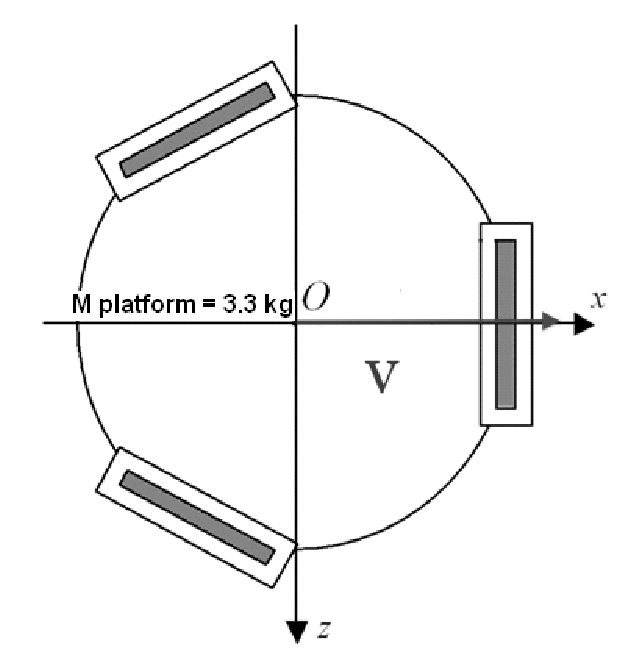
\includegraphics[width=7cm]{Translat.eps}
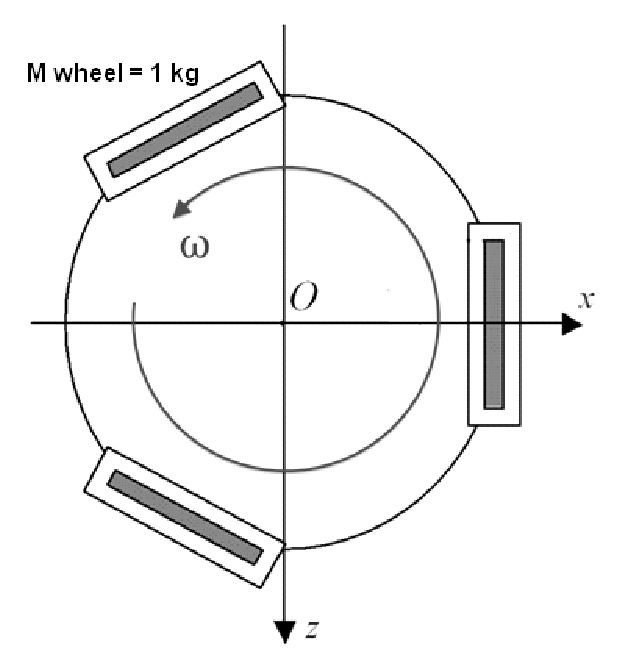
\includegraphics[width=7cm]{Rotat.eps}
}
\caption{Типы движения при верификации модели.}
\label{TypesOfMotion}
\end{figure}

Заметим, что перед началом процесса редукции индекса системы 
дифференциально-алгебраических уравнений полной модели экипажа, реализованного
в программном обеспечении лаборатории динамического моделирования 
Dymola~\cite{Dymola}, эта модель составляется из: а) твердого тела платформы
омни--экипажа; б) трех твердых тел --- моделей омни--колес; в) двенадцати 
твердых тел роликов, размещенных на колесах. В соответствии, например, 
с~\cite{Kosenko2007} для каждого объекта, моделирующего твердое тело, 
реализуются шесть обыкновенных дифференциальных уравнений (ОДУ) Ньютона для
движения центра масс тела плюс семь ОДУ Эйлера для вращательного движения тела
вокруг центра масс. В последнем случае имеется четыре кинематических уравнения
Эйлера для кватерниона ориентации тела плюс три динамических уравнения Эйлера
для вектора угловой скорости твердого тела. В результате полная модель экипажа
задается системой ОДУ порядка $16\cdot 13=208$. Кроме этого, объекты 
механических связей могут генерировать дополнительные дифференциальные 
уравнения.

Колеса, собранные в экипаж, с неизбежностью будут сохранять вертикальное 
положение. Поэтому упрощенный алгоритм отслеживания контакта, описанный выше,
всегда будет работать правильно. Численные эксперименты проводились для 
различных режимов движения экипажа: а) чисто поступательного --- движения 
корпуса из~Рис.~\ref{TypesOfMotion} вправо, б) чисто вращательного --- вращения 
корпуса вокруг вертикальной оси, проходящей через центр корпуса экипажа. 

%\begin{figure}[ht]
%\centerline{
%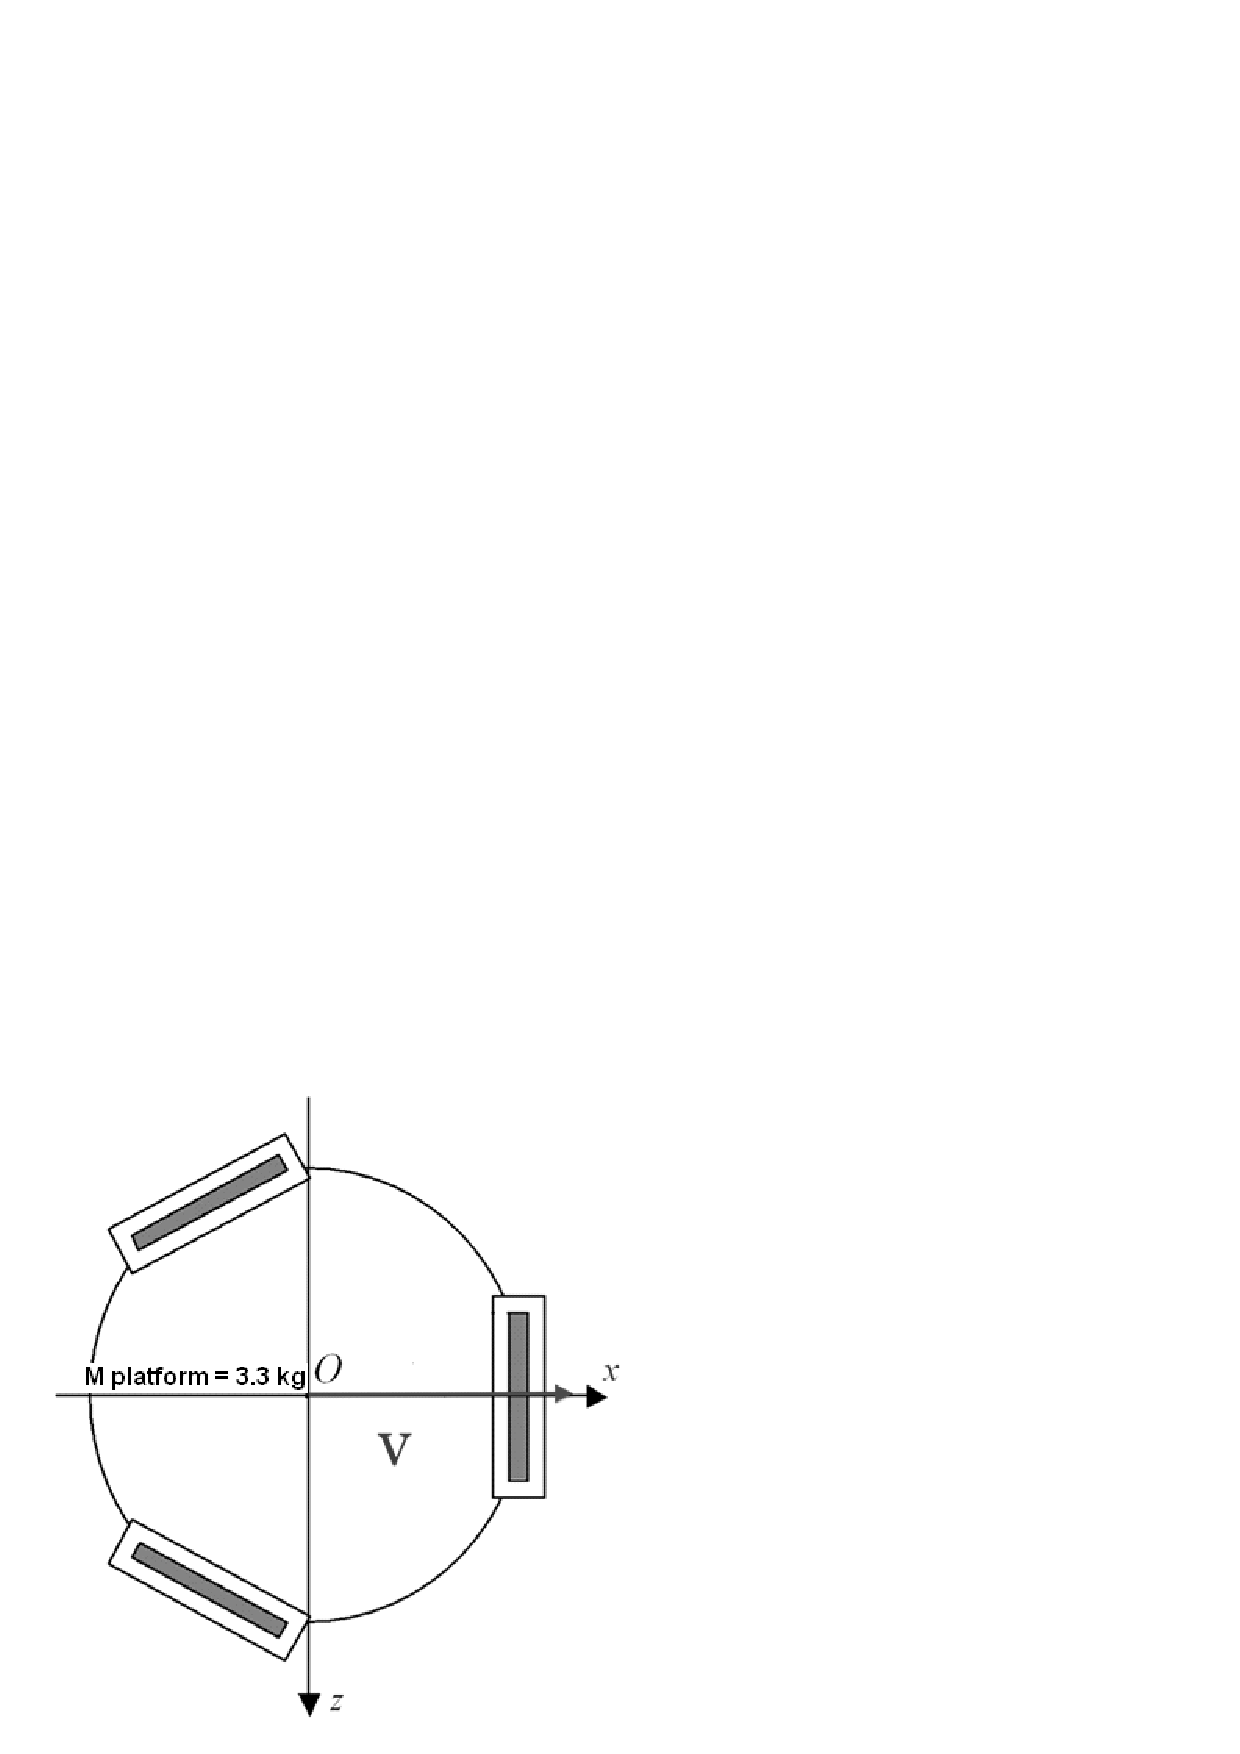
\includegraphics[bb= 0cm 0cm 10cm 10cm,scale=0.7]{Translat.png}
%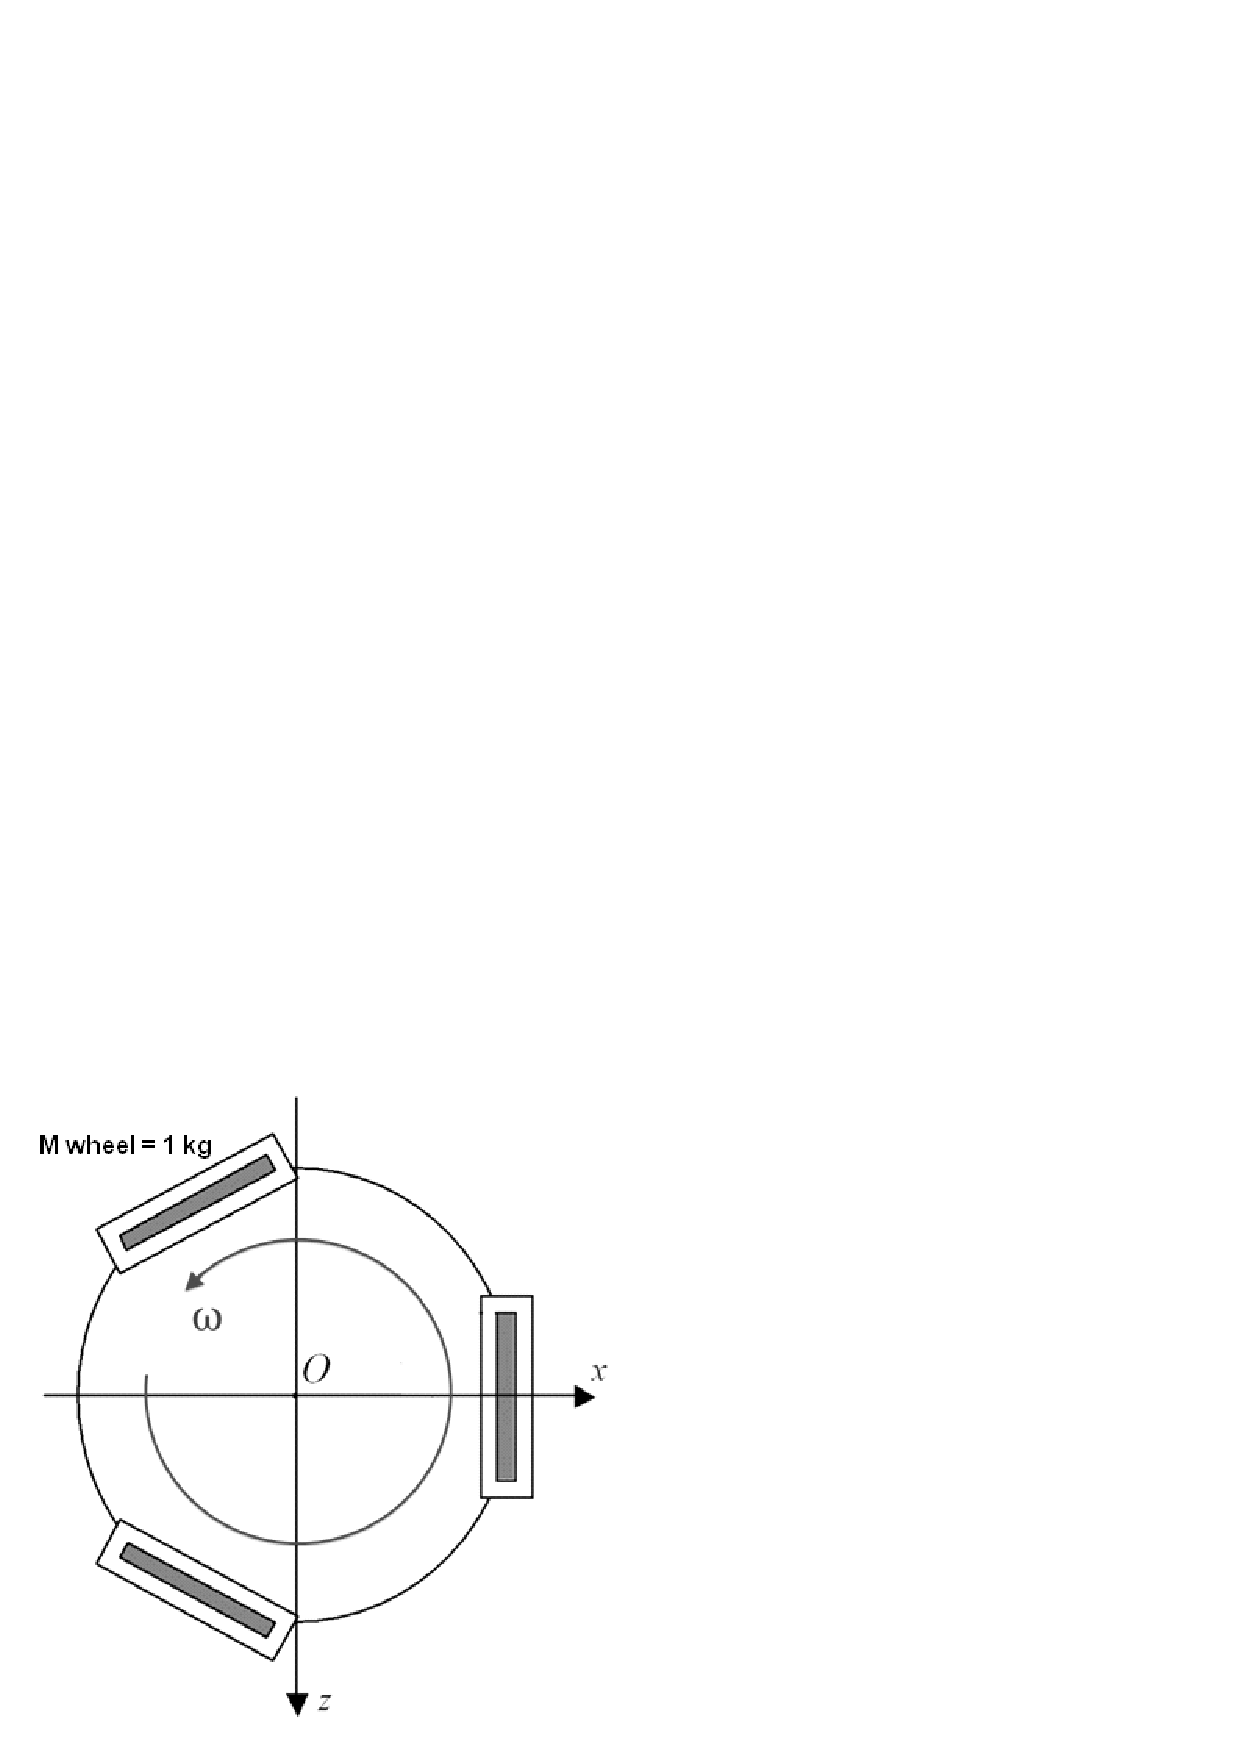
\includegraphics[bb= 0cm 0cm 10cm 10cm,scale=0.7]{Rotat.png}
%}
%\caption{Типы движения при верификации модели.}
%\label{TypesOfMotion}
%\end{figure}

Испытания проводились, в частности, и для случая, когда относительная суммарная 
масса роликов приближается к нулю. В этом случае оказалось, что движение 
экипажа и омни-колес неограниченно приближаются к соответствующим функциям 
решения задачи Коши, получаемым в силу дифференциальных уравнений движения, 
используемых в работе~\cite{BorisovKilinMamaev}, в которых динамика роликов не 
учитывается.

\begin{figure}[htb]
\centerline{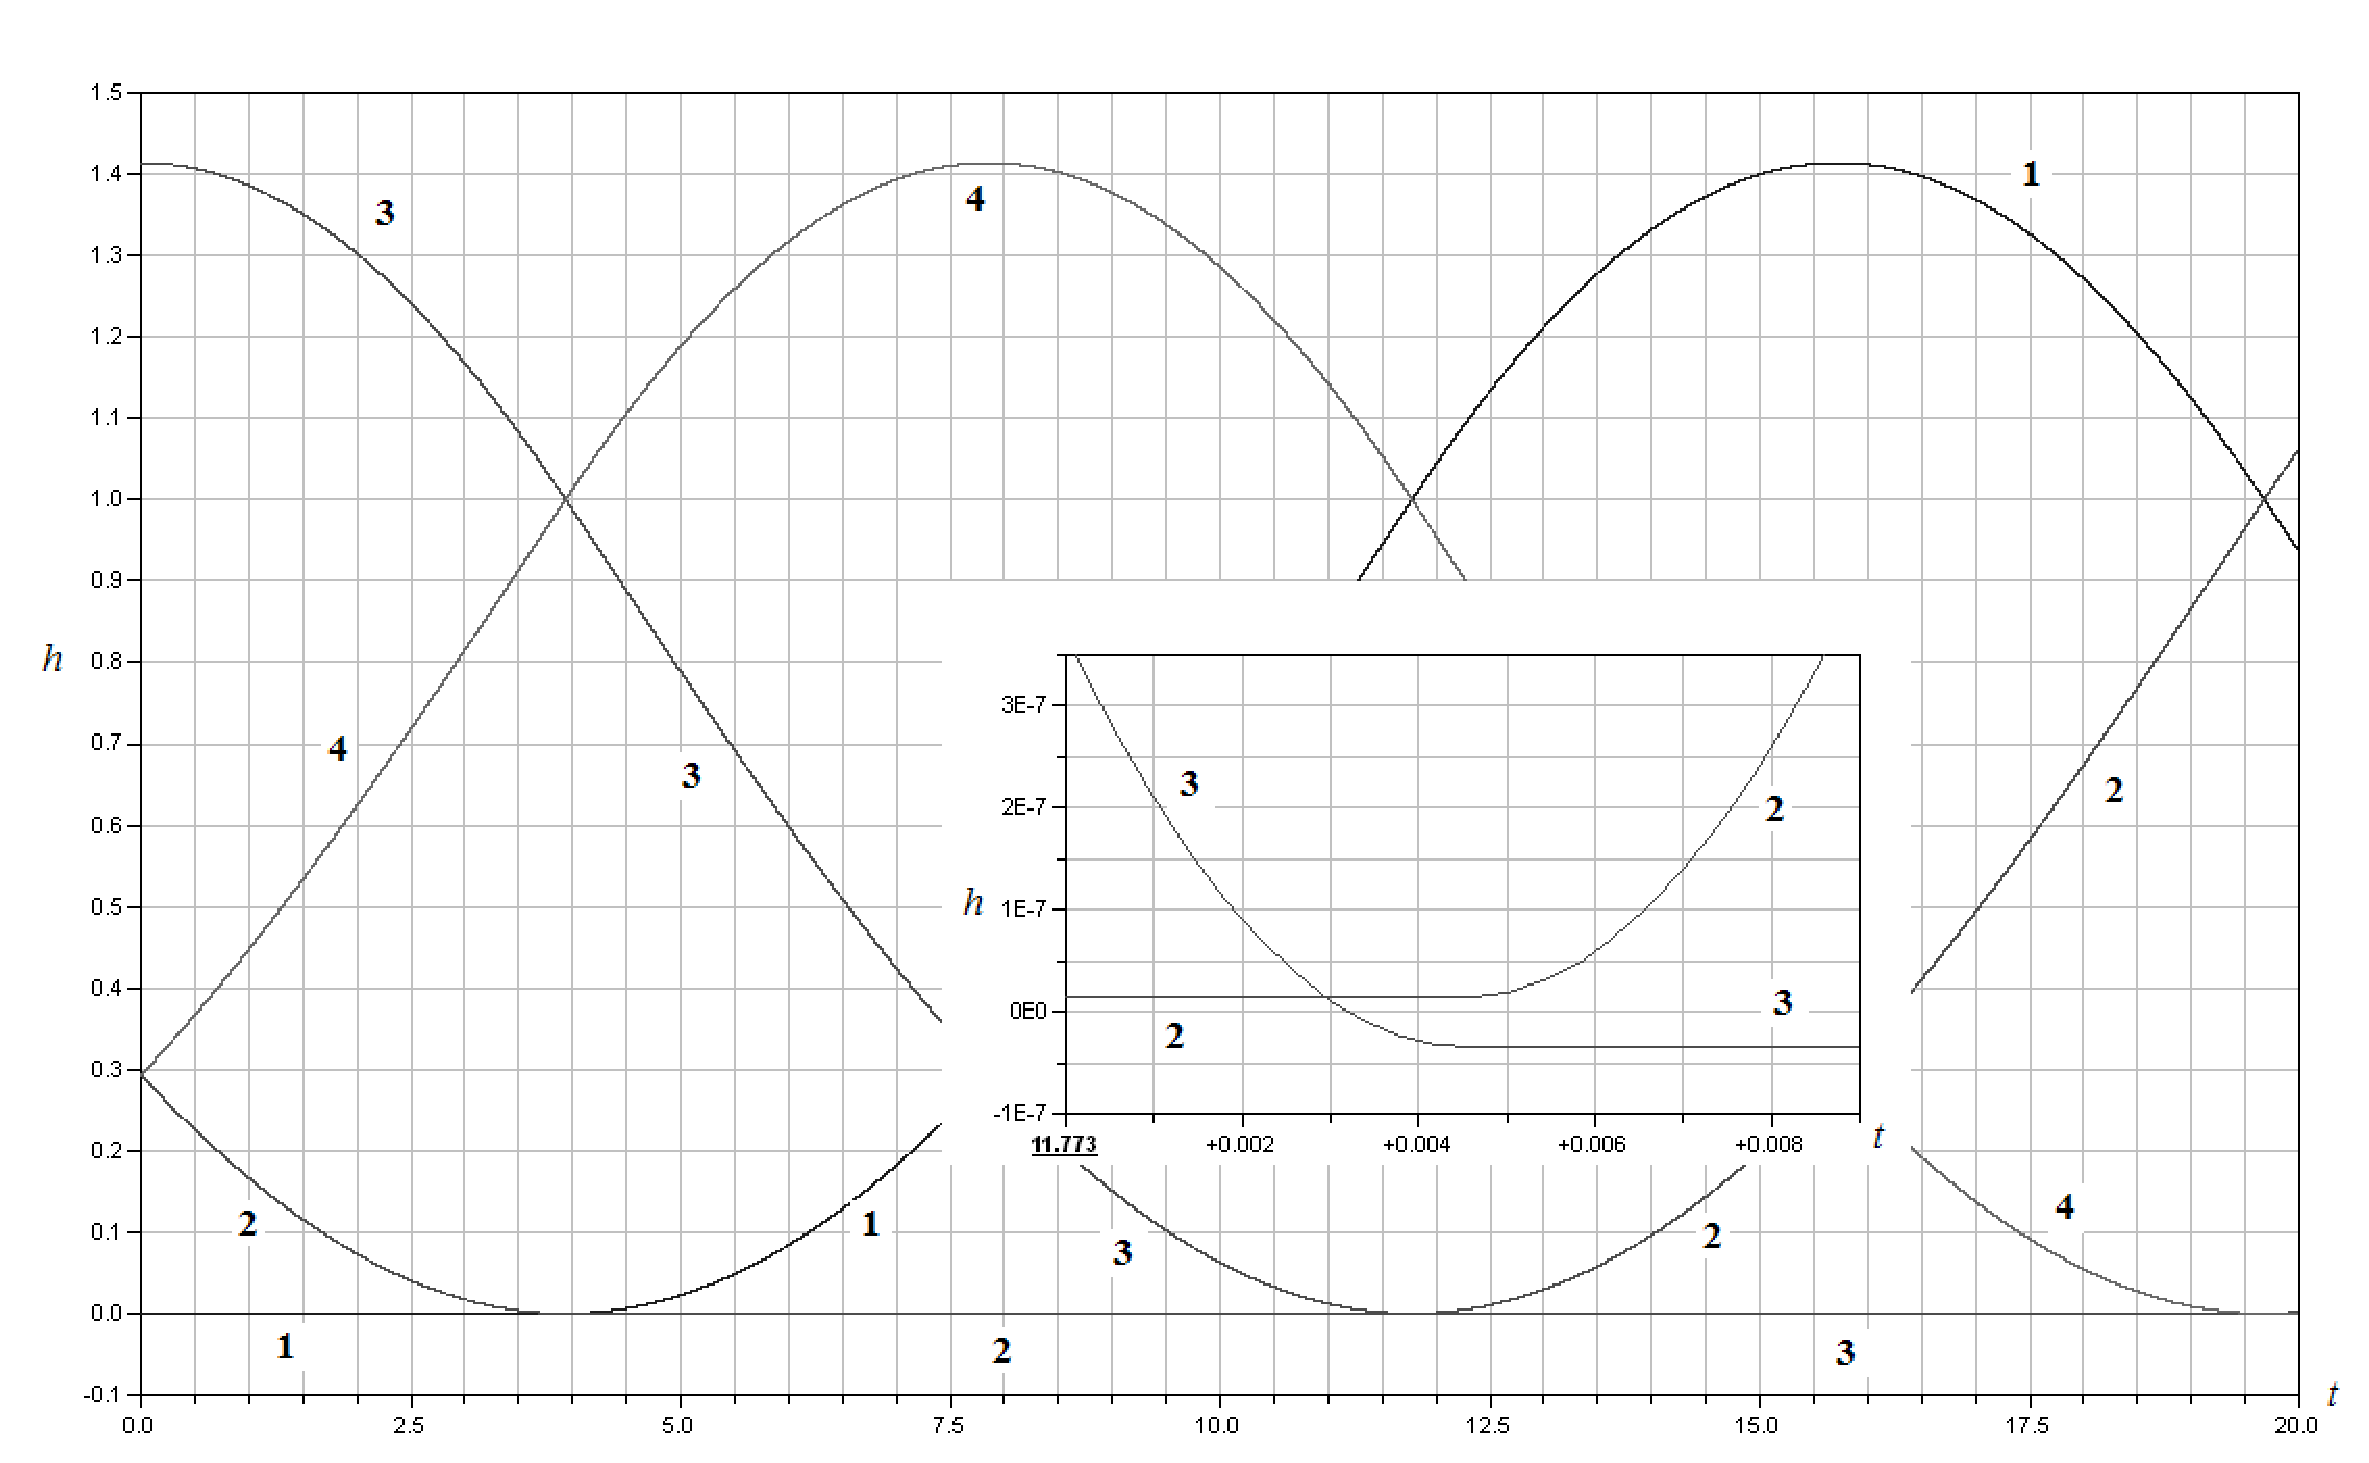
\includegraphics[width=15cm]{Figure11.eps}}
\caption{Процесс замещения роликов в контакте.}
\label{fig1}
\end{figure}

Эволюция процесса контактирования для отдельного катящегося омни-колеса 
показана на Рис.~\ref{fig1}, где представлены зависимости функций расстояний 
$h$ (фактически --- высот) между горизонтальной плоскостью (полом) и роликами 
одного и того же колеса, находящимися в разных фазах (перед контактом, в 
контакте, после контакта). Функция высоты отдельного ролика помечена номером 
этого ролика. В увеличенном масштабе показан момент безударного гладкого 
переключения поверхностей контактирования роликов и горизонтальной плоскости.
%\begin{figure}[ht]
%\centerline{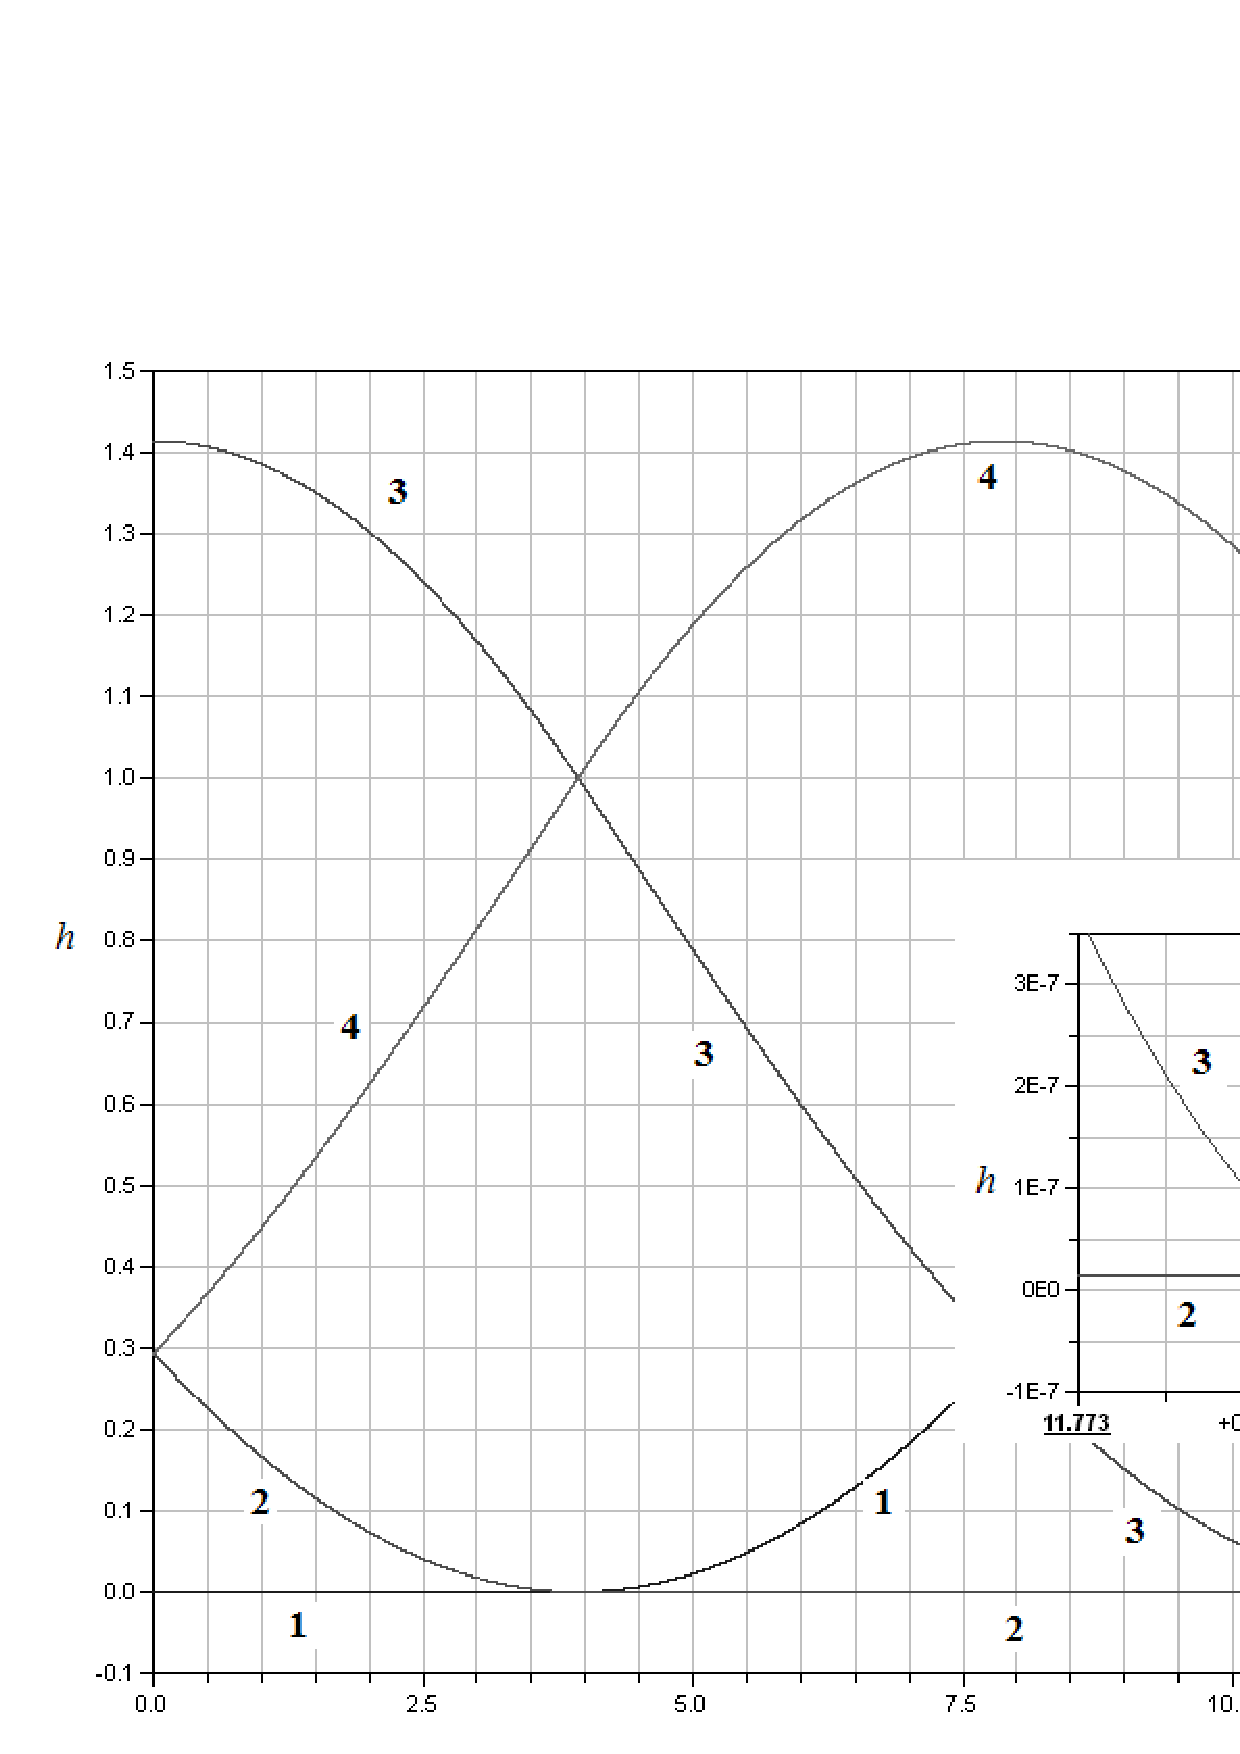
\includegraphics[bb= 0cm 0cm 20cm 12cm,scale=0.8]{Figure11.png}}
%\caption{Процесс замещения роликов в контакте.}
%\label{fig1}
%\end{figure}

Одновременно можно наблюдать точность соблюдения неудерживающей связи 
(Рис.~\ref{fig2}). Здесь обнаруживается процесс постепенного <<расползания>>
вычислительной ошибки --- расстояние между контактирующими телами медленно, для
каждого последующего ролика в контакте, увеличивается. В то же время, 
абсолютная величина ошибки остается пренебрежимо малой --- около $10^{-7}$
от единицы длины.
%\begin{figure}[ht]
%\centerline{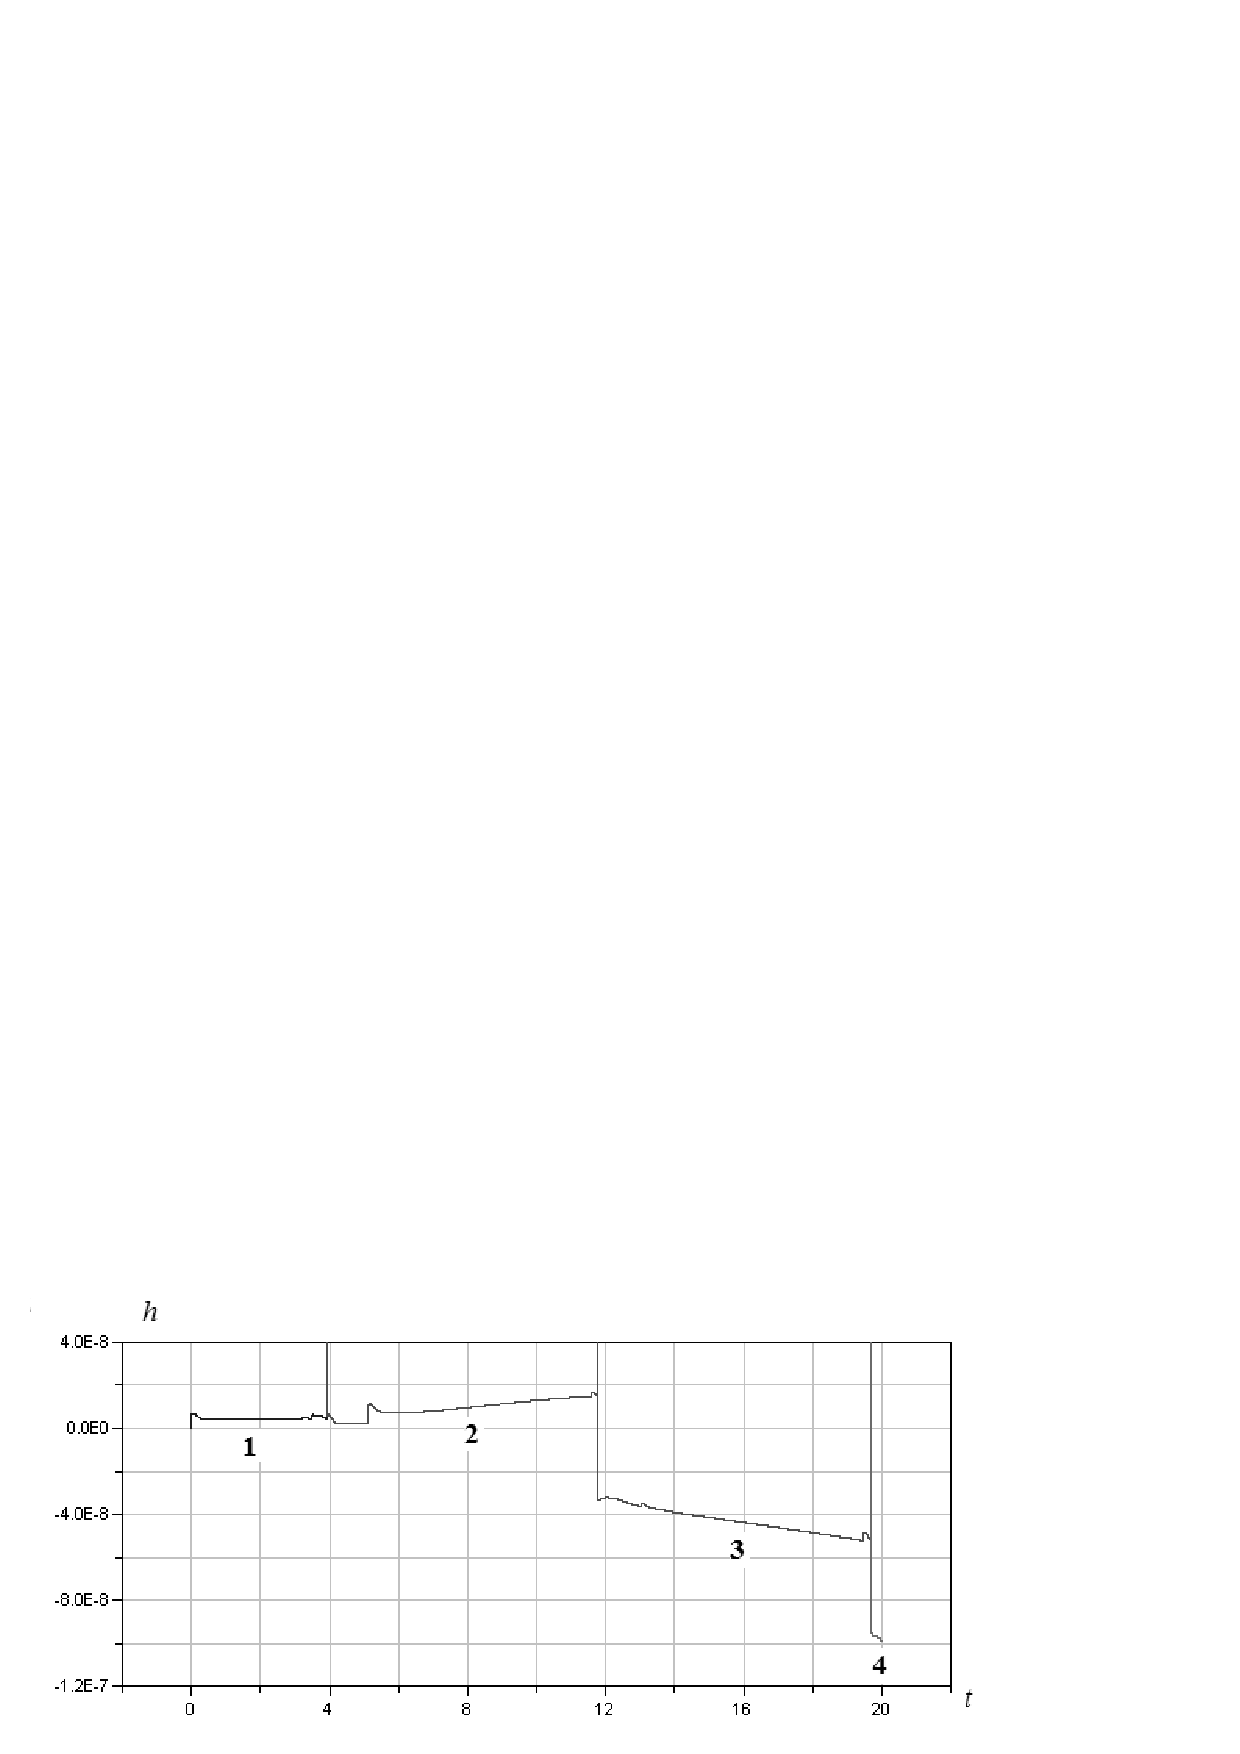
\includegraphics[bb= 0cm 0cm 20cm 8.5cm,scale=0.6]{Figure21.png}}
%\caption{Точность сохранения неудерживающей связи.}
%\label{fig2}
%\end{figure}
\begin{figure}[htb]
\centerline{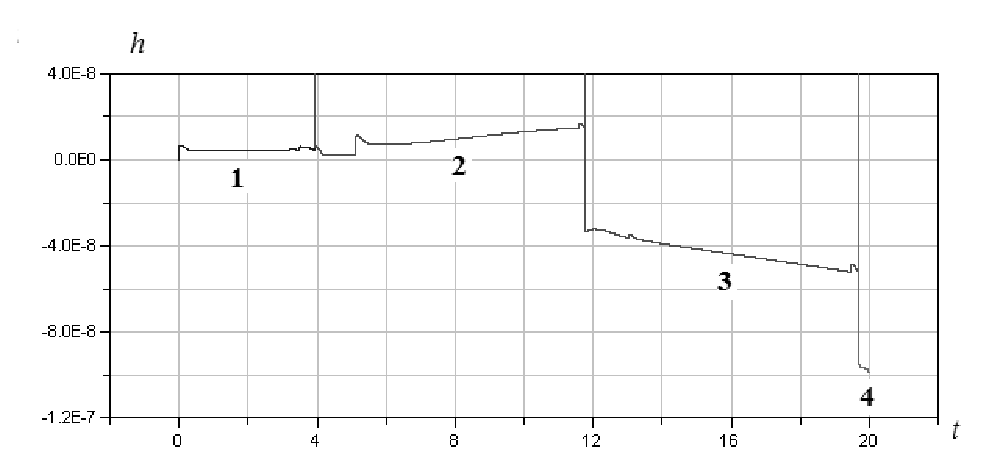
\includegraphics[width=15cm]{Figure21.eps}}
\caption{Точность сохранения неудерживающей связи.}
\label{fig2}
\end{figure}

\section{Выводы.\ }

В итоге построение виртуального прототипа (компьютерной модели) омни--экипажа 
позволило получить следующие результаты:
\begin{enumerate}

\item
Существует возможность гладкого безударного переключения роликов в контакте в
процессе качения/скольжения омни--колеса;

\item
Реализован упрощенный (и эффективный) алгоритм отслеживания контакта ролика и 
горизонтальной плоскости;

\item
Выполнена верификация динамической модели омни--экипажа с использованием 
модели, рассмотренной в работе~\cite{BorisovKilinMamaev}, в качестве 
предельного случая (когда суммарная масса роликов равна нулю).

\end{enumerate}

Работа выполнена в Московском авиационном институте (Национальном 
исследовательском университете) при финансовой поддержке Российского
научного фонда (проект № 14-21-00068).

\bigskip
\bigskip

\begin{thebibliography}{99}

\Russian
\bibitem{BorisovKilinMamaev}
Борисов А. В., Килин А. А., Мамаев И. С. Тележка с омниколесами на плоскости и 
сфере // Нелинейная динамика, 2011, т.~7, №~4, с.~785--801.

\bibitem{ZobovaTatarinov}
Зобова А. А., Татаринов Я. В. Динамика экипажа с роликонесущими колесами // 
Прикладная математика и механика, 2009, т.~73, вып.~1, с.~13--22.

\bibitem{Kosenko}
Косенко И. И. Интегрирование уравнений вращательного движения твердого тела в 
алгебре кватернионов. Случай Эйлера // Прикладная математика и механика, 1998, 
т.~62, вып.~2, с.~206--214.

\bibitem{Kosenko2006}
Косенко И. И. Реализация компьютерной модели динамики систем твердых тел с 
освобождающими связями // Математическое моделирование, 2006, т.~18, №~2, 
с.~95--106.

\bibitem{KosenkoAlexandrov}
Косенко И. И., Александров Е. Б. Реализация модели Контенсу -- Эрисмана 
касательных сил в контактной задаче Герца // Нелинейная динамика, 2009, т.~5. 
№~4, с.~499--517.

\bibitem{KosenkoGusev}
Косенко И. И., Гусев И. К. Компьютерная модель динамики прямозубого 
эвольвентного зацепления в редукторах // Нелинейная динамика, 2012. т.~8. №~4. 
с.~713--734.

\bibitem{KosenkoKuznetzova}
Моделирование и виртуальное прототипирование: учебное пособие / И.~И.~Косенко 
[и др.]. -- М.: Альфа-М : ИНФРА-М – 2012. 176~с.

\bibitem{Novozhilov}
Новожилов И. В., Фракционный анализ. Москва: Изд-во механико-математического
факультета МГУ, 1995. 224~с.

\English
\bibitem{CampionBastinAndreaNovel}
Campion G., Bastin G., d'Andr\'ea-Novel B. Structural Properties and 
Classification of Kinematic and Dynamic Models of Wheeled Mobile Robots // IEEE 
Transactions on Robotics and Automation, 1996, vol.~12, no.~1, pp.~47--62,

\bibitem{Dymola}
\url{http://www.3ds.com/products-services/catia/products/dymola}

\bibitem{Fritzson}
Fritzson P. Principles of Object--Oriented Modeling and Simulation with 
Modelica 2.1. Piscataway, New Jersey: IEEE Press, 2004. 898pp.

\bibitem{Kalman}
K\'alm\'an V. Controlled Braking for Omnidirectional Wheels // International 
Journal of Control Science and Engineering, 2013, vol.~3, no.~2, pp.~48--57.

\bibitem{Kosenko2007}
Kosenko I. I., Physically Oriented Approach to Construct Multibody System 
Dynamics Models Using Modelica Language // Proc. of Multibody 2007, Multibody 
Dynamics 2007. An ECCOMAS Thematic Conference (Politecnico di Milano, Milano, 
Italy, June 25--28, 2007), 20~pp.

\bibitem{Tobolar}
Tobol\'ar J., Herrmann F., B\"unte T. Object-Oriented Modelling and Control 
of Vehicles with Omni-Directional Wheels // Computational Mechanics 2009 (Hrad 
Nectiny, Czech Republic, November 9--11, 2009).

\end{thebibliography}

\newpage

\English

{\noindent\bf Physically-oriented simulation of the omni-vehicle dynamics}

\smallskip

\small
\noindent{Ivan. I. Kosenko${}^1$, Kirill. V. Gerasimov${}^2$}

\smallskip

\noindent ${}^1$Moscow Aviation Institute (National Research University),
Volokolamskoe shosse 4, 125993, Moscow, Russia\\
\noindent\url{kosenko@ccas.ru}

\noindent ${}^2$Lomonosov Moscow State University, 
GSP-1, 1-52, Leninskie gory, 119991, Moscow, Russia\\
\noindent\url{kiriger@gmail.com}

\smallskip
         
\normalsize

\noindent
Omni wheel is defined as one having rollers along its rim. Respectively omni 
vehicle is one equipped by omni wheels. Several steps of development of 
dynamical model of the omni vehicle multibody system are implemented. 
Initially, dynamics of the free roller moving in a field of gravity and having 
a unilateral rigid contact constraint with horizontal surface is modeled. The 
contact tracking using simplified and efficient algorithm turns out being 
possible. On the next stage the omni wheel model is implemented. After that the 
whole vehicle model is assembled as a container class having arrays of objects 
as instantiated classes / models of omni wheels and joints. Dynamical 
properties of the resulting model are illustrated via numerical experiments.

\smallskip

\noindent
\MSCindex{00A71 68U20 70E18 70E55 74H15 74M10 74M15 74M20} 
\noindent 
Keywords: omni-wheel; contact tracking algorithm; unilateral constraint; 
contact detection; friction model; object-oriented modeling 

\end{document}
